% !TEX encoding = UTF-8 Unicode
%\documentclass[12pt,reqno]{amsart}
\documentclass{article}
%\usepackage{tocloft}

%\cftsetindents{section}{0.5in}{0.5in}
%\cftsetindents{subsection}{0.5in}{0.5in}
\usepackage[utf8]{inputenc}
%\usepackage[dvips]{graphicx,graphics}
\usepackage{enumitem}
\usepackage{listings}
\usepackage{xcolor}
\definecolor{dkgreen}{rgb}{0,0.6,0}
\definecolor{gray}{rgb}{0.4,0.4,0.4}
\usepackage{graphicx}
\usepackage{euscript}
\usepackage{graphics}
%\usepackage{russcorr}
\usepackage[active]{srcltx} % SRC Specials: DVI [Inverse] Search
\usepackage{amssymb,amsmath,amsthm,amsfonts}
\usepackage{amsopn}
\usepackage{a4wide}
\usepackage{verbatim}
\usepackage{hyperref}
\usepackage{nameref}
\hypersetup{
    colorlinks,
    citecolor=black,
    filecolor=black,
    linkcolor=blue,
    urlcolor=blue
}
\usepackage{titlesec}
\titleformat{\section}[block]{\color{blue}\Large\bfseries\filcenter}{\thesection.}{1em}{}
\titleformat{\subsection}[hang]{\color{blue}\large\filcenter}{\thesubsection.}{1em}{}

\setlist[itemize,1]{leftmargin=\dimexpr 26pt+.3in}
\usepackage{a4wide}
\lstset{language=C++,
                basicstyle=\ttfamily,
		frame=tb,
		  aboveskip=3mm,
		  belowskip=3mm,
		  numberstyle=\tiny\color{gray},
		  keywordstyle=\color{blue},
		  commentstyle=\color{dkgreen},
		  stringstyle=\color{red},
		  breaklines=true,
		  breakatwhitespace=true,
		  tabsize=3,
                morecomment=[l][\color{magenta}]{\#}
}
\newcommand*{\fullref}[1]{\hyperref[{#1}]{\ref*{#1}. \nameref*{#1}}}
\begin{document}

%\begin{center} \hyperlink{debug}{\Huge{DEBUG}}\end{center}

\begin{center}
 \Large{\bf RAST: highly distributed DB project.}

{\large {\bf Produced by NOA team}}
\end{center}

\tableofcontents

\newpage
\section{Coding patterns}
\subsection{Function specifications cascade merging}
\label{subsec:specifications_cascade_merging}

Let us assume we are to write some template class, which may be customized with any amount of template parameters. Then, of course, we have to use variadic templates. When using variadic templates, we are to define class through its older version with less amount of template arguments, thus forcing compiler to produce a code for several hierarchical classes. What is often used here is so called cascade inheritance. That is, new class which is specified by a larger amount of template parameters is being inherited from an older version.

Imagine that we want target class $X<A,B,C>$ to have a template function, which has concrete specifications for template parameters being equal to $A$, $B$ or $C$. For instance, all classes $A$, $B$ and $C$ have $Output$ method and we want class $X$ to have $Output<T>$ method which for $[T=A]$ calls $Output$ method from class $A$, for $[T=B]$ calls $Output$ method of class $B$, etc.

First difficulty we would face considering such approach is that template specifications are not allowed in non-global scope (inside class $X$, for instance). That is due to the fact, that if those specifications depend on template parameters of $X$ class itself, the more complicated version of template processing algorithm would be required to handle this. But, template processing is not that smart enough to guess what author meant here. So, we have to specialize functions another way.

Let us do specifications by means of input arguments. In order to do so let us introduce an empty template class $TypeSpecifier<T>$. We may now write three versions of function, which compiler would treat well:

\begin{lstlisting}
class X {
public:
	void Output(const TypeSpecifier<A>&) {
		A().Output();
	}
	void Output(const TypeSpecifier<B>&) {
		B().Output();
	}
	void Output(const TypeSpecifier<C>&) {
		C().Output();
	}
};
\end{lstlisting}
Such a function would be called as follows:

\begin{lstlisting}
x.Output(TypeSpecifier<A>());
x.Output(TypeSpecifier<B>());
x.Output(TypeSpecifier<C>());
\end{lstlisting}
What remains is to represent this code using template processing:

\begin{lstlisting}
template <typename ... Args>
class X {
public:
	void Output() {}
};

template <typename T, typename ... Args>
class X<T, Args...>: public X<Args...> {
public:
	using X<Args...>::Output;
	void Output(const TypeSpecifier<T>&) {
		T().Output();
	}
};
\end{lstlisting}
By means of ``using'' construction we add all versions of Output function from previous inheritance level to the next one, afterwards adding new version associated with current new template parameter T. As far as we put ``using Output'' inside the code, we have to define ``Output'' symbol inside very base class, which accepts zero template parameters. In order to do that, we firstly define version of class ``X'', which accepts any amount of template arguments. The trick is that such implementation would only be considered if only ``X'' was zero template arguments, otherwise the declaration $X<T, Args...>$ would be chosen by compiler to process.

The only drawback here is that a user of the class has to know about some ``TypeSpecifier'' class to use ``Output'' function. But this can be fixed by introducing a final template function:

\begin{lstlisting}
template <typename ... Args>
class X {
public:
	void Output() {}
};
template <typename T, typename ... Args>
class X<T, Args...>: public X<Args...> {
public:
	using X<Args...>::Output;
	void Output(const TypeSpecifier<T>&) {
		T().Output();
	}
	template <typename T2>
	void TemplateOutput() {
		Output(TypeSpecifier<T2>());
	}
};
\end{lstlisting}

Now a call to ``Output'' function looks as follows:
\begin{lstlisting}
x.TemplateOutput<A>();
x.TemplateOutput<B>();
x.TemplateOutput<C>();
\end{lstlisting}

That is what is called ``cascade merging of specifications'' here.

The example on which technique is explained is rather simple and it would be weird to write such a complicated code, because one would just do something like this:
\begin{lstlisting}
template <typename T>
void Output() {
	T().Output();
}
\end{lstlisting}
In that, in the example above there was no actual need in inheritance, the example is just used in order to demonstrate the pattern. But when is this pattern really needed then?

A situation where such a complicated technique starts to be useful is when custom function needs to know something about the moment template argument was being added to template variadic list. That is, when in such a ``Output'' function we have to access a specific inheritance level. Imagine, for instance, that in class $X<A,B,C>$ we want to have a function $GetIndex$, which would by class name $A$, $B$ or $C$ return an index $2$, $1$ or $0$. To do it we have to store somewhere a correspondence between classes and indices. The best place for this is an inherited class:

\begin{lstlisting}
template <typename ... Args>
class X {
public:
	X()
	: max_index(0)
	{}

	void GetIndexImpl() {}
protected:
	int max_index;
};

template <typename T, typename ... Args>
class X<T, Args...>: public X<Args...> {
public:
	using X<Args...>::GetIndexImpl;
    using X<Args...>::max_index;

	X()
	: inheritance_level_index(max_index++)
	{}

	int GetIndexImpl(const TypeSpecifier<T>&) {
		return inheritance_level_index;
	}

	template <typename T2>
	int GetIndex() {
		return GetIndexImpl(TypeSpecifier<T2>());
	}
private:
	int inheritance_level_index;
};
\end{lstlisting}
That we have basically done here is incrementing ``inheritance\_level\_index'' in instantiation of each hierarchical class object, thus having increasing indices in the inheritance chain. Afterwards, while user is calling $GetIndex<T>$ function, the corresponding ``GetIndexImpl'' from the corresponding inheritance level would be called, and this function has a direct access to all the data stored in the level of inheritance it was defined. Thus, it can easily return the required index.

\subsection{Reverse template instantiation}
\label{subsec:reverse_template_instantiation}

In the section \fullref{subsec:specifications_cascade_merging} we have learned how to access data inside specific inherited class in the inheritance chain by given type name. Now assume the inverse task: given class $X<A,B,C>$ we want it to have a function Output(const int n) which calls ``Output'' function of $n-th$ class. That is, $Output(0)$ calls $C::Output$, $Output(1)$ calls $B::Output$, etc.

First and the simplest idea would be to do recursive calls until reaching needed inheritance level, and afterwards call the required ``Output'' function:
\begin{lstlisting}
template <typename ... Args>
class X {
public:
	X()
	: max_index(0)
	{}

	void Output(const int) {}
protected:
	int max_index;
};
template <typename T, typename ... Args>
class X<T, Args...>: public X<Args...> {
public:
    using X<Args...>::max_index;

	X()
	: inheritance_level_index(max_index++)
	{}

	void Output(const int index) {
		if (inheritance_level_index == index) {
			T().Output();
		} else {
			X<Args...>::Output(index);
		}
	}
private:
	int inheritance_level_index;
};
\end{lstlisting}
However, the drawback of such an approach is obvious: we do a lot of recursive calls, while another strategy would help up to avoid it. To cope with the task without recursive calls, we should have a fast way of accessing former ancestor classes. Let us store all hierarchical instances in vector then. But we cannot store instances of class ``X'' itself for the reason that it would result in infinite recursion depth if we would call instantiation of ``X'' class inside itself. Consequently, we have to use another class-helper ``Y'' the following way:
\begin{lstlisting}
template <typename ... Args>
class X {
protected:
    class Y {
    public:
        virtual void OutputImpl() {}
    };
public:
	X()
	{}

	virtual void OutputImpl() {}
protected:
	std::vector<Y *> instances;
};
template <typename T, typename ... Args>
class X<T, Args...>: public X<Args...> {
private:
    class Y : public X<>::Y {
        public:
            void OutputImpl() {
                T().Output();
            }
    };
public:
    using X<Args...>::instances;

	X()
    : X<Args...>()
	{
		instances.push_back(new Y());
	}


	void Output(const int index) {
		instances[index]->OutputImpl();
	}
};
\end{lstlisting}
Here in the constructor we initialize instances for each level of inheritance. Now we may access each level using this vector and use dynamic function resolution to call concrete ``OutputTmpl'' function, which does the job.

Imagine a more complicated situation, where function defined in ``A'', ``B'' or ``C'' classes may want to have access to $X<A,B,C>$ caller instance. For example, we want ``Output'' function of class ``C'' to accept the caller $x$ of type $X<A,B,C>$ and call $x.Output(1)$ in order to trigger $B::Output$. The problem here is that $Output(1)$, which triggers $C::Output$, is processed by $X<C>$ class in inheritance chain. That is why, it is quite unclear how do we manage to pass $X<A,B,C>$ instance to $C::Output$.

One of the most efficient ways to let parent know about a forthcoming child type is to use templates. Let us introduce a template subclass $Y<GlobalX>$, which is going to be defined inside ``X''. The aim is to make ``GlobalX`` template be replaced by $X<A,B,C>$ somehow during compilation process. To accomplish this let us again build up a vector of ``Y'' instances, but this time a vector will be constructed not during initialization, but rather after all hierarchical instances are ready, so that we could pass a last one as a template parameter. Let the initialization be in separate function called ``LazyInit''.
\begin{lstlisting}
template <typename ... Args>
class X {
public:
	template <typename GlobalX>
	class Y{
    public:
		Y(GlobalX& x)
		: x(x)
		{}

		virtual void Output() {}
	protected:
		GlobalX& x;
	};

	X()
	{}

    template <typename GlobalX>
    void LazyInitImpl(GlobalX&, std::vector<X::Y<GlobalX>*>&) {}
};

template <typename T, typename ... Args>
class X<T, Args...>: public X<Args...> {
public:
	template <typename GlobalX>
	class Y : public X<>::template Y<GlobalX> {
    public:
		using X<>::template Y<GlobalX>::Y;
        using X<>::template Y<GlobalX>::x;

		void Output() {
			T().template Output<GlobalX>(x);
		}
	};

	template <typename GlobalX>
	void LazyInitImpl(GlobalX& x, std::vector<X<>::Y<GlobalX>*>& y_hierarchical_instances) {
		X<Args...>::template LazyInitImpl<GlobalX>(x, y_hierarchical_instances);
		y_hierarchical_instances.push_back(new Y<GlobalX>(x));
	}

	void LazyInit() {
		LazyInitImpl<X>(*this, y_hierarchical_instances);
	}

	X<>::template Y<X>* GetYInstance(const int index) {
		return y_hierarchical_instances[index];
	}
private:
	std::vector<X<>::template Y<X>*> y_hierarchical_instances;
};
\end{lstlisting}
Usage of this class would be as follows:

\begin{lstlisting}
class A {
public:
    template <typename GlobalX>
    void Output(GlobalX& x) {
        std::cout << "This is A!\n";
    }
};
class B {
public:
    template <typename GlobalX>
    void Output(GlobalX& x) {
        std::cout << "This is B!\n";
    }
};
class C {
public:
    template <typename GlobalX>
    void Output(GlobalX& x) {
        std::cout << "This is C!\n";
        x.GetYInstance(1)->Output();
    }
};


int main() {
    X<A,B,C> x;
    x.LazyInit();
    x.GetYInstance(0)->Output();
    return 0;
}
\end{lstlisting}
Note that now classes ``A'', ``B'' and ``C'' are able to use $x$ instance. Yet, as far as these classes does not know about $x$ type, their ``Output'' function has to be template.

Now, with the usage of ``reverse template instantiation'' pattern we are able to access methods of classes by index and to access external controller class object inside each of the class passed as a template parameter.

\newpage
\section{Algorithmic basis}

\subsection{Free-list multi-level allocator}
\label{free_list_algo}

On of the most important steps in order to make a low-latency system is to consider the allocation problem. The problem is that sometimes different components of the program require very small parts of memory to be allocated. Asking the system to allocate memory directly would result in slower performance. That's why it is better to allocate large memory segment and distribute its parts among several consumers.

But here we face another difficulty, so called fragmentation problem. Imagine that an allocated segment is separated into several parts owned by consumers. Some time after, some of the consumers returned their own parts to allocator (calling deallocate method). Afterwards it appears that the returned memory in control of allocator is represented as distinct small fragments. Those fragments cannot be given to a consumer, who asks for a larger memory segment, than the size of the separate fragment. If there is a lot of such unusable fragments, we would have a lot of memory allocated, which will never be used. In order to avoid this problem, we have to force each small fragment to be used by a consumer who asks for a small amount of memory.

The main idea is to use a memory levels.

\begin{center}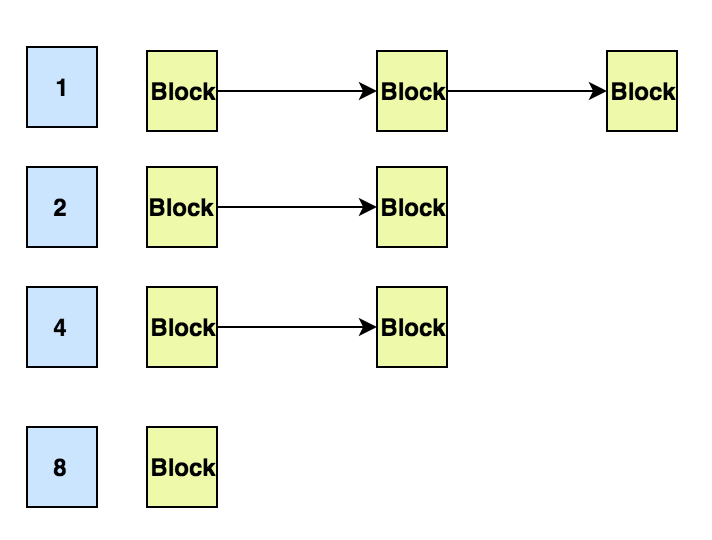
\includegraphics[width=0.5 \textwidth]{image1.png}\end{center}

For each block size we calculate an integer part of $log(size)$ and put all blocks of memory in the corresponding list.

By means of the list, we can easily find the block of needed size and remove (detach) it from the list, giving ownership to the consumer, who asked to allocate memory. Likewise, when a consumer asks to deallocate the block, we may put (attach) it again in the list.

Also we want to join small segments of memory returned by consumers to one large segment in case if they go one after another in the global memory space. In order to do this, let us have the following structure of the memory block:

\begin{center}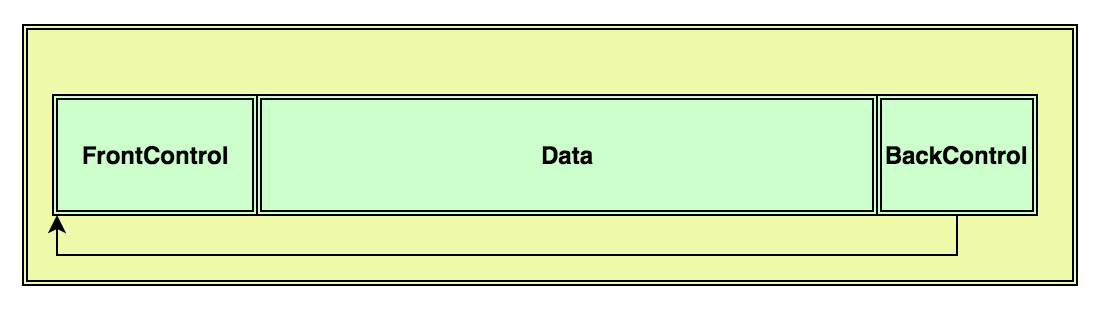
\includegraphics[width=0.5 \textwidth]{image2.png}\end{center}

The block will consist of three logical parts:
\begin{itemize}
\item FrontControl, which stores the $data\_size$ which is size of the block, $localnext$ and $localprev$ pointers, $offset$ in external allocated segment, and $total\_size$ of external segment, and $is\_owned$ -- whether the block is owned by the allocator itself or was it given away to the consumer.
\item Data -- raw byte space, which would be given an external consumer to control
\item BackControl, which stores pointer to the FrontControl (pointer to the beginning of the entire block)
\end{itemize}

$localprev$ and $localnext$ pointers will help us to build freelists, which were described above. BackControl block will help us to find the block, previous to some specific Block, so that we could join two blocks together in case they both have been returned to the allocator. Here is how joining procedure works:

\begin{center}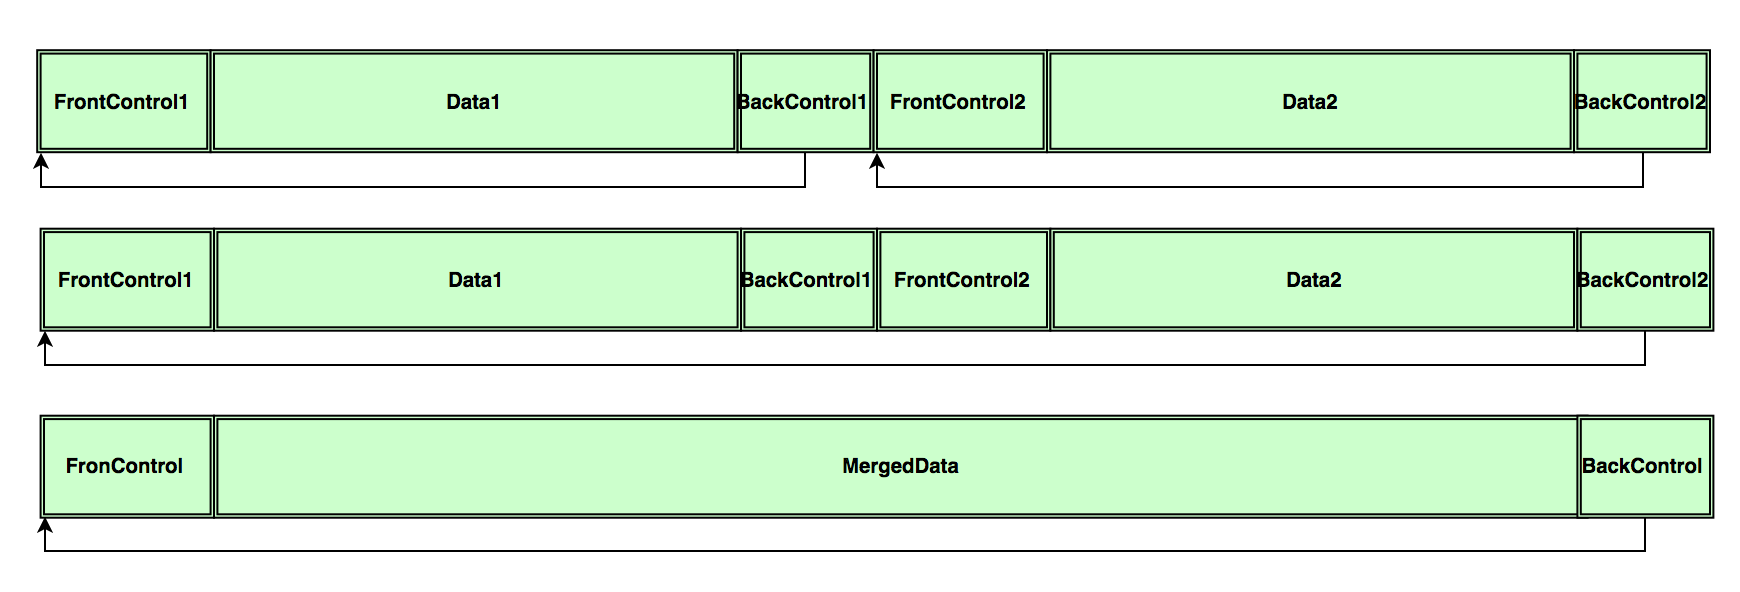
\includegraphics[width=1 \textwidth]{image3.png}\end{center}

The steps are very simple:

\begin{itemize}
\item detach first block from its list
\item detach second block from its list
\item point BackControl2 to FrontControl1
\item change FrontControl1 information about block size
\item do nothing about BackControl1 and FrontControl2, because now we threat them as a garbage part of MergedData, and we do not have to care about their contents so far
\item attach new merged block to its new list (based on $log(size)$ where $size$ is a sum of sizes of these two blocks) by changing $localprev$ and $localnext$ pointers of FrontControl.
\end{itemize}

Also, one can easily imagine how to split one large block into two smaller.

Blocks contained in the same external memory segment (which allocator asked from the system) may be joined and split so that we know exactly how many consequent free to use bytespace fragments do we have.

Finally, the allocation procedure is the following:

\begin{itemize}
\item calculate integral part $N = int(log(size))$ of the size of the memory consumer asks to allocate
\item if the corresponding $N$-th list of blocks is empty, we allocate several external blocks of the sizes $2^{N}$ and build Block structure upon each of them, putting blocks to the $N$-th list
\item detach first block from the list
\item split the block into two blocks: first block has exactly needed size, second block consists of what is remained
\item attach second block to its corresponding list
\item mark the first block as not owned by allocator
\item return a pointer to the Data section of the first block to a consumer
\end{itemize}

The deallocation procedure:
\begin{itemize}
\item receive from a consumer a pointer to deallocate data
\item calculate the pointer to FrontControl (by subtracting $sizeof(FrontControl)$ from Data pointer)
\item mark block as owned by the allocator
\item read $offset$ from FrontControl, if $offset > 0$, than there is some previous block in the external memory segment.
\item calculate the pointer to BackControl of the previous block (by subtracting $sizeof(BackControl)$ from the pointer to the current block)
\item get the pointer to the FrontControl of the previous block via BackControl
\item check whether the previous block is owned by the allocator and if it is, merge it with the current block
\item if $offset < total\_size$ where $total\_size$ is the size of external allocated memory segment, we may want to check whether we can merge with the forthcoming block
\item calculate the pointer to the FrontControl of the forthcoming block (by adding $data\_size + sizeof(FrontControl) + sizeof(BackControl)$ to the pointer to the current block)
\item check if the forthcoming block is owned by allocator using its FrontControl and if it is, merge it with the current block.
\end{itemize}
\newpage

\subsection{Lock-free queue (without deallocations)}
\label{subsec:lock_free_queue}

Queue is a basic container, which is often desired to be used in more or less complicated systems. Although queue implementation is very simple, it is not thread-safe. In order to make it thread-safe, one may decide to use mutexes in Pop and Push operations. The idea is not good enough for several reasons:
\begin{itemize}
	\item all threads would compete against each other for gaining control over mutex,
	\item all kernels would have to sync the mutex state via cache ping-pong, which would lead to plenty of time waisted on system calls,
	\item jobs of threads would be serialized, that is, the queue is 100\% not scalable.
\end{itemize}

The main idea is that if we get down to the details of queue implementation, we may reorganize it in such a way, that we would not need to have mutually exclusive access to guarantee that each operation works fine. That is, we may obtain a lock-free algorithm on the queue.

In order to do that, let us represent queue as a linked list, each node of each except for the last one, contains data elements. The last node, which is the tail of the queue would not contain any data at all. Let us call it a dumb node:

\begin{center}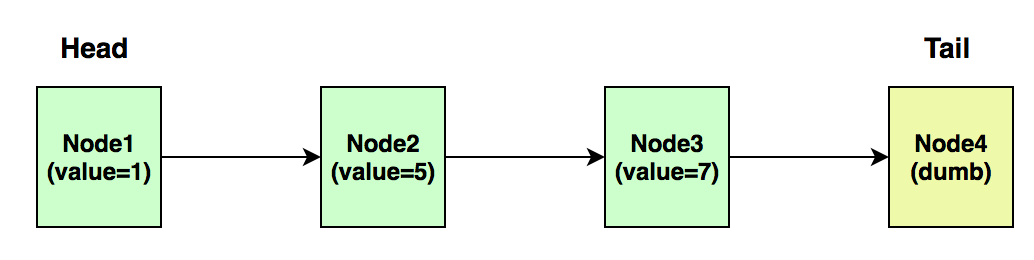
\includegraphics[width=0.5 \textwidth]{image4.png}\end{center}

Head, Tail and Next pointers inside data structure would be atomic pointers, which would be changed using CAS operations. The main idea of Push is:
\begin{itemize}
	\item put new data to the dumb node
	\item create another dumb node and mark it as a tail
\end{itemize}

But these are two distinct actions, which are not guarded by mutual exclusion and thus are not atomic. So, by choosing this strategy we should agree that it is OK for the queue to be one of the following two:

\begin{center}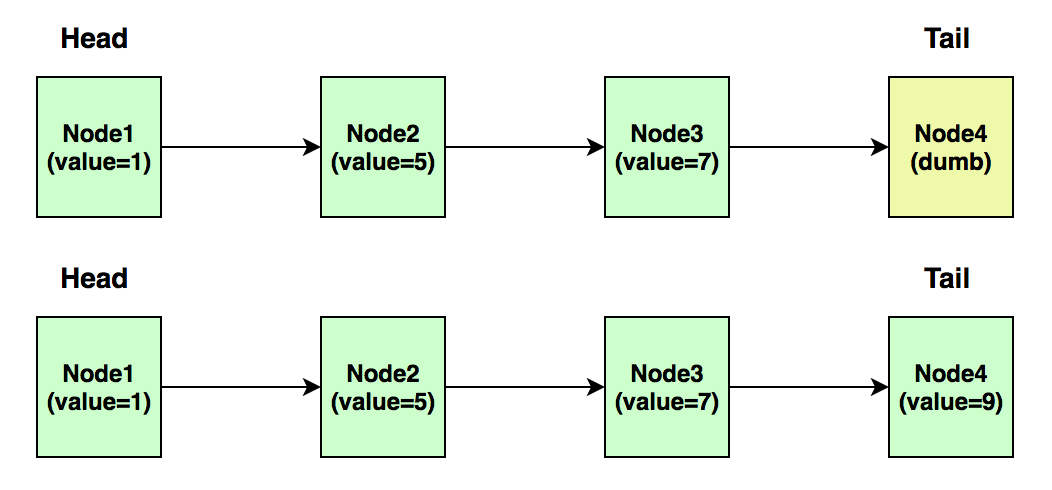
\includegraphics[width=0.5 \textwidth]{image5.png}\end{center}

That is, we agree on purpose that queue may either have dumb element or not have dumb element. But if it is like that, we have to redesign Push:

\begin{itemize}
	\item try CAS data on the tail (nullptr $\rightarrow$ our new data)
	\item if CAS succeeded, the queue actually had a dumb node and now we may proceed to adding a new dumb node
	\item if CAS failed, the queue does not have a dumb element, so we firstly create a dumb node as a tail, and retry the algorithm from the start
\end{itemize}


Changing tail pointer is also a CAS operation, but in case if it fails, we realize that another thread have already moved tail forward and thus we do not have to do anything, so we will not process tail CAS operation failure on purpose without harming algorithm invariants at all.

The detailed version of Push consists of the following steps:
\begin{itemize}
	\item allocate new data
	\item allocate new dumb node
	\item L1: load tail
	\item L2: try CAS tail.data (nullptr $\rightarrow$ allocated new data)
	\item L3: if L2 succeeded, try CAS tail.next (nullptr $\rightarrow$ new dumb node)
	\item if L3 failed, somebody already moved tail.next to new node, so deallocate new dumb node, try CAS tail (old\_tail $\rightarrow$ value of tail.next), ignore the results and finish Push
	\item if L3 succeeded, try CAS tail (old\_tail $\rightarrow$ new dumb node), do not care about results and finish Push
	\item L4: if L2 failed, we do not have dumb node in the end of the queue, try CAS tail.next (nullptr $\rightarrow$ new dumb node)
	\item if L4 succeeded, we shall allocate new dumb node, try CAS tail (old\_tail $\rightarrow$ value of tail.next), ignore the result of this operation and repeat algorithm from L1 point
	\item if L4 failed, try CAS tail (old\_tail $\rightarrow$ value of tail.next), ignore the result of this operation and repeat algorithm from L1 point using the same already-allocated new dumb node
\end{itemize}

Note that the only action among these which may throw is an allocation, but all allocations happen-before successful L2 step. That is, in case if L2 succeeded, the rest of the code in Push in exception-free. Success of L2 operation means that new data is put to the queue, failure means that the data was not put to the queue yet. This implies we are having strong exception safety on Push operation: if it throws, it would surely mean that data was not put to the queue. This is the best available exception guarantee (after "noexcept") for a queue user. Of course, guaranteeing noexcept is impossible, because no one can imagine Push operation without memory allocations, which always may throw.

Now let us consider Pop operation. It would check if head is equal to tail. If it is, the queue consists of dumb node only, thus there is no data. In this case Pop would return empty unique\_ptr. In the other case, we will switch the head to the next element, giving away first node data.

The detailed version of Pop consists of the following steps:
\begin{itemize}
	\item read head, tail
	\item L1: check head == tail
	\item if L1 is true, return empty unique\_ptr
	\item L2: if L1 is false, do CAS head (current $\rightarrow$ next)
	\item if L2 failed, retry from the start
	\item if L2 succeeded, store and exchange data from old head, return it to the caller
\end{itemize}

%\begin{center} \hypertarget{debug}{\Huge{DEBUG}}\end{center}
Notice that Pop is exception-free.

The implementation described here does not do deallocations, which poses a memory leak problem. The problem is handled in the forthcoming section \fullref{subsec:dealloc_lock_free_queue}.

\subsection{Multi-counters deallocation technique}
\label{subsec:three_counters}

Almost any algorithm underlaying some lock-free data structure requires careful deallocation technique. The \hyperref[subsec:lock_free_queue]{algorithm of lock-free queue} we have described above is not an exclusion. The implementation considered does not deallocate memory at all, thus suffering from a memory leak.

The simple but not correct approach is to deallocate node, which is being popped. The problem here is that we have to provide strict guarantee that no other thread is still working with data, which current thread is going to return to the memory heap.

More complicated, but still not correct idea is to count references to the node. We increase reference count if we are going to use a node, and decrease when it is no longer needed. And when counter hits zero, we are going to deallocate the data. Unfortunately, this attempt to write thread-safe deallocation code would also fail, because the counter being equal zero at some point of time does not guarantee that it would be zero the next moment of time. This implies, that checking whether the counter is zero is a useless operation: after checking conditional has passed, and we moved forward to deallocating data, some other thread could ask for one more copy of the object and increase reference count by 1. But, as far as in the current thread we have already decided to deallocate memory, we no longer care about reference counter value. The result is a race condition in the code, which again leads to the fact that some thread uses memory another thread is going to deallocate.

The most complicated, and this time, absolutely correct option, is to always bear in mind reference counter, but start to attempt comparing it with zero and deallocating memory only after the moment when we can guarantee that no other reference to the object is going to be created in the future. That is, we wait until the user-written code somehow manages to say ``I will no longer create new references on this specific data''. After this moment, we start to wait until user-written code stops to use existing (created before this moment) references. And after that, we may freely deallocate the memory, without any races.

In a more general case, there are several users, which may produce copies of the references to the object. Then reference counting mechanism should receive a promise not to create copies in the future from each one of them. In order to do that, we would use $external\_counters$ variable. At the initialization point, it stores the number of sources, which can produce copies of references to the object. Once a source tells that it would no longer produce copies, the $external\_counters$ decreases. Than it equals zero, we start trying to deallocate the data.

In order to store reference count, we introduce $internal\_counter$, which is stored in the data itself. Apart from that, each source, which can create reference copies, would contain $external\_counter$ -- a number of reference copies it created on specific data.

Let us call source, which has not yet promised not to create copies of references, an $active$ source. In our three-counter approach the following invariant would hold: for each data element sum of  $internal\_counter$ and all $external\_counter$ values of all active sources is equal to reference count to this data.

To sum up, data element contains $internal\_counter$ and $external\_counters$ inside itself, while each reference to the data element consists of the pointer as well as $external\_counter$.

Now we have to define several procedures.

The access protocol:
\begin{itemize}
	\item source, which want to copy reference, increases its $external\_counter$
	\item ... some operations over data element ...
	\item send data element a command to decrease its $internal\_counter$
\end{itemize}

Source nocopy promise:
\begin{itemize}
	\item send a data element command to atomically decrease $external\_counters$ and to increment $internal\_counter$ by the value of $external\_counter$ of the current source
\end{itemize}

The cleaning condition:
\begin{itemize}
	\item if  $internal\_counter$ and $external\_counters$ of data element are both equal zero, deallocate the data
\end{itemize}

This condition is checked both on the finish of the access protocol and after receiving nocopy promise and if true, data is deallocated.

It is very simple to prove that all the operations described keep invariant that sum of $internal\_counter$ and all $external\_counter$ values of all active sources is equal to reference count. Because of that, cleaning condition is proven to be true. Indeed, if $external\_counters$ equals zero, all sources promised not to create copies in the future. Therefore, by that moment there are no active sources, that is, $internal\_counter$ (summed up with nothing) now stores the exact amount of references left. And, of course, if it also equals zero, then all access protocols are complete. That surely implies we can deallocate data with no problems.

There are also a few rather important details about the implementation:
\begin{itemize}
	\item $internal\_counter$ and $external\_counters$ are stored in the data element itself and should mutate atomically and simultaneously. This can be lock-free only on processors, which support DWCAS.
	\item $external\_counter$ and pointer to the data element should also be packed to the one structure and mutate using DWCAS
	\item all operations described are exception-free, which means that the method can be used in any data structure without harming exception guarantees of the data structure itself.
	\item in order to simplify matters in the access protocol, we would incapsulate copying in the constructor of special CopyGuard class, and incapsulate decreasing $internal\_counter$ in its destructor.
\end{itemize}

\subsection{Multi-counters lock-free queue (final algorithm)}
\label{subsec:dealloc_lock_free_queue}

Here we are to combine the ideas in \fullref{subsec:lock_free_queue} and \fullref{subsec:three_counters}.

Now the node of the queue is going to contain its $internal\_counter$ and $external\_counters$. In the queue we also need several atomic variables, which point to the nodes: head, tail and next. Let the head, tail and next be objects, which contain $external\_counter$ and a pointer to the node.

Also, head, tail and next would be associated with three sources, which may produce reference copies. It is required for the correct usage of access protocol, because we would have to access head, tail and next pointers in our algorithm, and the only way to access data element is to duplicate its reference.

While where to use an access protocol and a cleaning condition is a rather simple question, we should consider when do we send nocopy promises.

For tail, we should send nocopy promise when tail is moved further than current data element. This implies that the current data element is never going to be a tail in the future, thus we may guarantee that reference on it cannot be copied from tail.

For next and head, we will send nocopy promise only when the data element is popped out of the queue. This would surely guarantee that no other head and next pointers will ever point to current data element in the future, and the corresponding references will never be copied.

The final implementation of Push operation:

\begin{itemize}
	\item allocate new data
	\item allocate new dumb node
	\item L1: copy tail using CopyGuard (forcing the increase of $external\_counter$)
	\item L2: try CAS tail.data (nullptr $\rightarrow$ allocated new data)
	\item L3: if L2 succeeded, try CAS tail.next (nullptr $\rightarrow$ new dumb node)
	\item if L3 failed, somebody already moved tail.next to new node, so deallocate new dumb node, try CAS tail (old\_tail $\rightarrow$ value of tail.next). If succeeded, send nocopy promise to the node. In any case finish Push.
	\item if L3 succeeded, try CAS tail (old\_tail $\rightarrow$ new dumb node). If succeeded, send nocopy promise to the node. In any case finish Push.
	\item L4: if L2 failed, we do not have dumb node in the end of the queue, try CAS tail.next (nullptr $\rightarrow$ new dumb node)
	\item if L4 succeeded, we shall allocate new dumb node, try CAS tail (old\_tail $\rightarrow$ value of tail.next). If succeeded, send nocopy promise to the node. In any case repeat algorithm from L1 point (CopyGuard destructor is called implicitly in the end of the cycle iteration, forcing the decrease of $internal\_counter$)
	\item if L4 failed, try CAS tail (old\_tail $\rightarrow$ value of tail.next). If succeeded, send nocopy promise to the node. In any case repeat algorithm from L1 point using the same already-allocated new dumb node (CopyGuard destructor will be called implicitly)
\end{itemize}

The final implementation of Pop operation:

\begin{itemize}
	\item copy head using CopyGuard
	\item L1: check head == tail
	\item copy head.next using CopyGuard
	\item if L1 is true, return empty unique\_ptr
	\item L2: if L1 is false, do CAS head (current $\rightarrow$ next)
	\item if L2 failed, retry from the start (CopyGuard destructors for head and next are called implicitly)
	\item if L2 succeeded, store and exchange data from old head
	\item trying until success to do CAS next (current\_value $\rightarrow$ nullptr\_special). It cannot hang for an infinite time, because, since the head have already been moved, no new calls to Pop will deal with this ``next'' pointer of popped head. This means, that we have to wait only finite amount of calls in another threads, which accidentally read same head to be popped, to finish. Threads, which have accidentally read the same head to be popped, would face L2 operation failure, and immediately after that would go to the start of algorithm, where they would reload another head. So, the threads, which may access the same popped head, would not be blocked, they would just go out of the way of the current thread and let it change ``next'' pointer. Threads, which do Pop, may also want to access current vertex in case if the queue is empty and tail == head. But they also cannot be blocked, because there is only one cycle in the Pop operation, which rereads data at the start, and the next iterations would not see already-popped head and would not interact with the ``next'' pointer in question. As all interactions with ``next'' would fade away after finite number of steps in finite number of threads, we would be able to do CAS successfully. That is why it is lock-free to wait until CAS next (current\_value $\rightarrow$ nullptr\_special) actually succeeds.
	\item after that, send nocopy promise of type ``next'' about the next element of the popped head (because it will never be someone's else next element, although may still be inside the queue)
	\item send nocopy promise of type ``head'' about the popped head (because it will never be a head again)
	\item return data from popped head to the caller (CopyGuard destructors are called implicitly)
\end{itemize}

What is specific about Pop operation is this weird nullptr\_special we used in CAS next. The matter of the fact is that to guarantee strictly that the node, contained in the ``next'' pointer, would never be copied, we have to assign ``next'' pointer to something else. Exactly this assignment, as have already been explained, waits for other threads, which want to operate with the same ``next'' pointer, to stop making ``next'' reference copies. Still there is a field for bug in the code. If we assign next to nullptr, we may open the ability for Push operation to change this ``next'' pointer, because Push operation does CAS next (nullptr $\rightarrow$ new dumb node). The Push operation is based on the idea that the only node, which has ``next'' pointer being equal to nullptr, is the tail node. By assigning nullptr to ``next'' pointer of the popped head, we corrupt this invariant and Push may attach new node to the popped node, which is totally unacceptable. Thus, if we want to change ``next'' pointer value, we cannot use nullptr for this purpose. But, we may use another special pointer value, which we are sure that nobody else uses. This is what is called a nullptr\_special here.

What is remained is to deallocate the rest of nodes of the queue in destructor. This is done by calling Pop a lot of times in the destructor (since Pop is noexcept, we may freely do so). Afterwards, the only dumb vertex remained, which cat be either deallocated directly, or we may send nocopy promises from head and tail and it would also be deallocated automatically by three-counters logic.

To summarize, we designed Push and Pop operations in such a way, that
\begin{itemize}
	\item all data allocated will at some point be deallocated
	\item all accessed data in each thread is protected and would not be deleted while read
	\item Push can throw, strong exception safety is still guaranteed for the reason that reference counting itself is exception-free and all guarantees from lock-free queue are preserved
	\item Pop is exception-free
\end{itemize}

\subsection{Multi-counters lock-free queue (productivity)}
\label{subsec:dealloc_lock_free_queue_productivity}

\hyperref[subsec:dealloc_lock_free_queue]{The algorithm of queue} appears to be so complex, that one may wonder: is it really faster than the queue, protected by mutex? Let us do a couple of tests to show the difference between these two implementations.

Imagine we have 4-processor hardware. Imagine there are two threads, one of which wants to send 10 million Pop requests, another wants to send 10 million Push requests.

In case of lock-free queue the result is the following:
\begin{lstlisting}
real    0m6.079s
user    0m11.314s
sys     0m0.077s
real RPS = 3.33 million
\end{lstlisting}

In case of mutex-protected queue the result is the following:
\begin{lstlisting}
real    0m5.500s
user    0m6.980s
sys     0m3.146s
real RPS = 3.63 million
\end{lstlisting}

One may think that it is not so impressive, because lock-free implementation was 0.5 seconds slower (real time). But a closer look will reveal, that
\begin{itemize}
	\item mutex-protected queue takes a lot of system time. Of course, it does, because a lot of time is required to synchronize very-fast-changing values of mutex bool flag. Because the threads compete for the ownership of the mutex, cache ping-pong is very likely to happen, forcing queue to be slower
	\item user time of lock-free queue is even bigger, 11.3 seconds, which is bad comparing with 6.9 seconds of mutex-protected version. But, from a scalability point of view, the lock-free implementation is far better. Using two threads, we gain almost ideal ratio of 11.3 seconds of user time and 6 seconds of real time. As for mutex-protected queue, we get almost no scalability, because each operation is protected with a mutex. Of course, this leads to a threads serialization, and we gain 6.9 seconds of user time resulting in 5.5 seconds of real time, which is a bad result for two-threaded program.
\end{itemize}
So, lock-free queue is slower, because it contains a lot more logic in its implementation. But, it does not spend so mush time on system calls and is ideally scalable.

Let us watch what is going to be if there are two threads, which try to Pop 10 million elements, and also two threads, which try to Push 10 million elements (4 threads in total).

In case of lock-free queue:
\begin{lstlisting}
real    0m10.082s
user    0m37.448s
sys     0m0.949s
real RPS = 4.0 million
\end{lstlisting}

In case of mutex-protected queue:
\begin{lstlisting}
real    0m17.316s
user    0m23.260s
sys     0m25.856s
real RPS = 2.3 million
\end{lstlisting}

So here we see the drawbacks of mutex-protected queue in action:
\begin{itemize}
	\item the system time increased dramatically, because now 4 threads and competing for single mutex, and its value needs to be synchronized to 4 processors instead of 2
	\item the scalability is still poor: we get 17.3 seconds of real time having 23.2 seconds of user time.
	\item mutex-protected queue degrades in RPS after we increased threads count: from 3.6 million queries per second to 2.3 million. That is quite a bad degradation.
\end{itemize}

And again we clearly see the advantages of lock-free queue:
\begin{itemize}
	\item it waists less than a second of system time, that is, almost 26 times less that mutex-protected queue. This means, it would not go slower if there would be a lot of another processes doing system calls
	\item it is still almost perfectly scalable: we get 10 seconds of real time having 37.4 seconds of user time, which is a good result for a 4-threaded application
	\item the user time of lock-free implementation still exceeds the user-time of mutex-protected queue (the fact that lock-free queue needs more time to execute its logic cannot be changed), but, due to scalability, real time shows that now, with 4 threads, it is almost 1.5 times faster than a mutex-protected implementation
	\item lock-free queue does not suffer from RPS degradation while we scale concurrency. It even became faster: from 3.33 million requests per second it increased up to 4 million requests per second. That is a very good result.
\end{itemize}

On the account of these simple measurements, we decided that it is better to use a lock-free algorithm.

\subsection{Low-overhead periodic timer}
\label{subsec:low_overhead_periodic_timer}

In order to make the system more efficient, sometimes it is required to measure operations in order to distribute them ideally between different threads. However, a lot of calls to system timer would result in slower performance.

The purpose of the current section is to establish easy-to-use time measuring algorithm, which will somehow not slow down the performance being called a lot of times in a short period of time. To simplify matters, let us construct a timer, which has $GetPassedTime$ function, which being called the first time, would return unix timestamp (time since year 1970), and being called further would return the time passed since its last call. Let us also have a $Reset$ method, which resets timer settings to default ones. This timer will not be thread-safe, it will be designed to be used in one thread only.

Basically, the idea is simple: if we cannot access system clock on each call, be should access them more rarely, thus sometimes we will provide approximate results on $GetPassedTime$ call. On the contrary, sometimes on $GetPassedTime$ call we will call system clock and catch up or slow down depending on our previous not exact responses. That is, our not-so-exact timer needs to be winded up when we do access system clock.

In order to do that let us introduce what information does such a timer store:
\begin{itemize}
	\item static constant $min\_system\_clock\_call\_period$ which is a minimal desired time, after which we want to call $WindUp$
	\item static constant $max\_wind\_up\_steps$ which tells how many calls of $GetPassedTime$ at maximum should be until next wind-up
	\item static constant $min\_measured\_time$ is a minimal value we would return from $GetPassedTime$ function
	\item $wind\_up\_counter$ is a counter, which decreases on each $GetPassedTime$ call and being equal zero forces winding up process
	\item $wind\_up\_balance$ is a difference between real time and sum of all times returned from $GetPassedTime$ during program execution
	\item $last\_wind\_up\_counter$ stores the value of counter, which was set just after last wind-up
	\item $last\_system\_time$ is system time measured while last wind up
	\item $approx\_time\_step$ is an approximate value, which is a prognosis of time elapsed since previous $GetPassedTime$ call
\end{itemize}

The initial values of parameters would be the following:
\begin{itemize}
	\item $wind\_up\_counter = 1$
	\item $wind\_up\_balance = 0$
	\item $last\_wind\_up\_counter = 1$
	\item $last\_system\_time = 0$
	\item $approx\_time\_step$ will be initialized on first $GetPassedTime$ call, as it will be seen further
\end{itemize}

The $Reset$ procedure would reset parameters to their initial values.

The $WindUp$ procedure would do the following:
\begin{itemize}
	\item store current system time in $system\_time$ variable
	\item calculate $time\_passed = system\_time - last\_system\_time$
	\item calculate $new\_wind\_up\_counter = max(1, \\min(min\_system\_clock\_call\_period / time\_passed * last\_wind\_up\_counter,\\ max\_wind\_up\_steps))$. That is, if $time\_passed$ is less than \\$min\_system\_clock\_call\_period$, we want to increase amount of calls we want to perform until next win-up by the ratio of these values. But, we do not want it to be more than $max\_wind\_up\_steps$ and less than 1.
	\item update $approx\_time\_step = time\_passed / last\_wind\_up\_counter +\\+ wind\_up\_balance / new\_wind\_up\_counter$
	\item update $last\_wind\_up\_counter = new\_wind\_up\_counter$ to store new last counter
	\item update $wind\_up\_counter = last\_wind\_up\_counter$ to do next wind up after this amount of steps
	\item update $last\_system\_time = system\_time$ to save result for future wind-up
	\item update $wind\_up\_balance += time\_passed$ in order to maintain $wind\_up\_balance$ invariant
\end{itemize}
Now let us consider the following algorithm for $GetPassedTime$ operation:
\begin{itemize}
	\item decrease $wind\_up\_counter$
	\item if $wind\_up\_counter$ equals zero, call $WindUp$ method
	\item calculate $result\_time = max(min\_measured\_time, approx\_time\_step)$
	\item update $wind\_up\_balance -= result\_time$ to maintain $wind\_up\_balance$ invariant
	\item return $result\_time$
\end{itemize}
During the first $GetPassedTime$, $WindUp$ would be called immediately and will initialize $approx\_time\_step$, which has already beed stated. And the initialization of $approx\_time\_step$ appears before its first usage.

Why is this supposed to be correct? First of all, imagine a situation when we call $GetPassedTime$ so rarely, that $time\_passed$ is large enough to be more than $min\_system\_clock\_call\_period$ and also more than $min\_measured\_time$, and $last\_wind\_up\_counter$ equals 1 and $wind\_up\_balance$ equals zero. Let us trace how parameters will be updated in $WindUp$ method:
\begin{itemize}
	\item store current system time in $system\_time$ variable
	\item calculate $time\_passed = system\_time - last\_system\_time$
	\item update $new\_wind\_up\_counter =\\= max(1, min(\\min\_system\_clock\_call\_period / time\_passed *\\* last\_wind\_up\_counter, max\_wind\_up\_steps)) =\\= max(1, min(0, max\_wind\_up\_steps)) = max(1, 0) = \\=1$.
	\item update $approx\_time\_step = time\_passed / last\_wind\_up\_counter +\\+ wind\_up\_balance / new\_wind\_up\_counter = time\_passed / 1 + 0 / 1 =\\= time\_passed$
	\item update $last\_wind\_up\_counter = new\_wind\_up\_counter = 1$
	\item update $wind\_up\_counter = last\_wind\_up\_counter = 1$ so $WindUp$ would be called on next $GetPassedTime$ call
	\item update $last\_system\_time = system\_time$ to save result for future wind-up
	\item update $wind\_up\_balance += time\_passed$ so $wind\_up\_balance$ would equal $time\_passed$ now
\end{itemize}
This way, $last\_wind\_up\_counter$ continues to be equal 1 and next time the same calculations would also hold. Now let us consider what will happen in $GetPassedTime$ procedure:
\begin{itemize}
	\item decrease $wind\_up\_counter$
	\item $wind\_up\_counter$ equals zero because it was being equal 1 before, so we definitely call $WindUp$ method
	\item $wind\_up\_balance$ equals $time\_passed$, as well as $approx\_time\_step$ does
	\item calculate $result\_time = max(min\_measured\_time, approx\_time\_step) =\\= max(min\_measured\_time, time\_passed) = time\_passed$, because we assumed that $time\_passed \geq min\_measured\_time$
	\item update $wind\_up\_balance -= result\_time$, which makes $wind\_up\_balance$ being equal zero again.
	\item return $result\_time$, which is equal to $time\_passed$
\end{itemize}
Thus, all values we assumed at the start ($last\_wind\_up\_counter = 1$, $wind\_up\_balance = 0$) would still remain the same after $GetPassedTime$ call. That is why, the same will repeat on the next $GetPassedTime$ call and it will always return correctly calculated precise $time\_passed$ result on each call. That is, in case of large enough $time\_passed$, our timer is equivalent to simple timer logic.

Another important point is that in any case we are trying to make $wind\_up\_balance$ being equal zero. Indeed, we set $approx\_time\_step = time\_passed / last\_wind\_up\_counter +\\+ wind\_up\_balance / new\_wind\_up\_counter$. Expression $time\_passed / last\_wind\_up\_counter$ evaluates to average time between $GetPassedTime$ previous calls. Expression \\$wind\_up\_balance / new\_wind\_up\_counter$ results in the fact, that during next $new\_wind\_up\_counter$ calls of $GetPassedTime$ we will, apart from main logic, decrease previous error $wind\_up\_balance$ to zero while updating $wind\_up\_balance -= result\_time$. Simultaneously, a new error, which the prognosis $time\_passed / last\_wind\_up\_counter$ poses, will also be accumulated while doing $wind\_up\_balance -= result\_time$, and it will be handled during the next $WindUp$ call, while we will count new $approx\_time\_step$.

$wind\_up\_balance$ parameter is rather important. It shows our overall accumulated calculation errors and if it is a large negative number, it implies that the sum of returned times from $GetPassedTime$ dramatically exceeded real time pace, and $approx\_time\_step$ would be negative in such a case, forcing $result\_time$ we give out to be equal $min\_measured\_time$. In case if $wind\_up\_balance$ is a rather big positive number, we will return larger values from $GetPassedTime$ because of larger $approx\_time\_step$, which would help us to catch up with the time pace.

Notice that $GetPassedTime$ is designed to be called exactly from one location in the code, because we use the fact that approximately same time passes between $GetPassedTime$ calls while calculating $time\_passed / last\_wind\_up\_counter$ as an expected virtual time step.

\subsection{Low-overhead start-finish timer}
\label{subsec:low_overhead_start_finish_timer}

Let us construct a timer, which would help to measure some code execution time. It would have $Start$ and $Finish$ methods, which are to be called before and after desired code block. Also it would have $GetCount$ method, which will return count of measurements, and $GetDurationSum$ method, which would return sum of all measured times. Moreover, there will be a $Reset$ method, which resets counters.

In order to avoid slow performance due to a lot of system timer calls, we will use \fullref{subsec:low_overhead_periodic_timer}.

Our timer object would store the following information:
\begin{itemize}
	\item $start\_timer$ which is a periodic timer associated with start event
	\item $finish\_timer$ which is a periodic timer associated with finish event
	\item $measurements\_counter$ which stores count of measurements
	\item $duration\_sum$ which stores sum of all durations measured so far
\end{itemize}

Now let us consider, what methods do.

Algorithm for $Start$ method:
\begin{itemize}
	\item decrease $duration\_sum$ by $start\_timer.GetPassedTime()$ (method $GetPassedTime$ is defined in the \fullref{subsec:low_overhead_periodic_timer} section)
\end{itemize}

Algorithm for $Finish$ method
\begin{itemize}
	\item increase $duration\_sum$ by $finish\_timer.GetPassedTime()$
	\item increase $measurements\_counter$
\end{itemize}

$GetCount$ method returns  $measurements\_counter$

$GetDurationSum$ method returns $max(PeriodicTimer::min\_measured\_time, duration\_sum)$.

$Reset$ method reinitializes all parameters $measurements\_counter$ and $duration\_sum$ and calls $Reset$ method of timers $start\_timer$ and $finish\_timer$.

The implementation here is very simple due to the fact that we have already passed through all the difficulties while building \fullref{subsec:low_overhead_periodic_timer} algorithm.

As far as \fullref{subsec:low_overhead_periodic_timer} has a unique caller requirement (must be called from one specific location in the code), our $Start$ and $Finish$ methods also have the same requirement.

\subsection{Low-overhead waiting timer}
\label{subsec:low_overhead_waiting_timer}
Here we are aiming to create a timer, which helps to schedule periodic actions. In constructor it accepts a time period value. It has $CheckTime$ function, which returns $true$ if given time passed, and $false$, if time have not passed yet. Also there would be a $Reset$ function, which resets waiting process from the start.

As far as there can be a lot of $CheckTime$ calls in a short period of time, the good idea would be to use \fullref{subsec:low_overhead_periodic_timer}.

Our $WaitingTimer$ would contain the following variables:
\begin{itemize}
	\item $time\_period$ which is set by user in $WaitingTimer$ constructor
	\item $time\_elapsed$ which is time passed after last $Reset$ call
	\item $periodic\_timer$
\end{itemize}

$Reset$ method has the following logic:
\begin{itemize}
	\item call $periodic\_timer.GetPassedTime()$ to fix point since which we are going to trace time
	\item update $time\_elapsed = 0$
\end{itemize}

$Reset$ should be called in the constructor of the class $WaitingTimer$.

Function $CheckTime$ would have the following logic:
\begin{itemize}
	\item update $time\_elapsed += periodic\_timer.GetPassedTime()$
	\item return evaluated condition $time\_elapsed > time\_period$
\end{itemize}

Now our method $CheckTime$ acts if it was planned. However, it bears a unique caller requirement as far as \fullref{subsec:low_overhead_periodic_timer} does.

\subsection{Low-overhead periodic clock}
\label{subsec:low_overhead_periodic_clock}

$PeriodicClock$ would be a class, which is called from one specific location in the code and helps to get approximate current time without doing system call each time.

It is based on \fullref{subsec:low_overhead_periodic_timer}

It would contain the following data:
\begin{itemize}
	\item $current\_time$
	\item $periodic\_timer$ of class $PeriodicTimer$
\end{itemize}

It would have the only method $GetTime$, which does the following:
\begin{itemize}
	\item increments $current\_time$ by value of $periodic\_timer.GetPassedTime()$
	\item returns $current\_time$
\end{itemize}

\subsection{Exception top proto storage}
\label{subsec:exception_top_proto_storage}
In order to make it simple for users to administrate the system, let us somehow notify users about exception thrown. Here we face a problem if some exception is thrown a lot of times, it becomes hard to distinguish it from other exceptions. Hence, it is better to store the same exception once with its appearance count. To avoid a lot of memory spent on storing exceptions, let us store only limited top of ones, since it is highly unlikely that any user would ever need to examine over thousand distinct exceptions without fixing the most frequent ones at first.

Let us introduce class $ExceptionTopKeeper$, which would help to update top of exceptions with their frequencies, save it on disk and restore it from disk. Our $ExceptionTopKeeper$ would not be thread-safe and has to be instantiated inside TLS. That is, each thread would have its own exceptions top and a specific place to store it.

$ExceptionTopKeeper$ contains the following data:
\begin{itemize}
	\item variable $path$, which is a path of a file where exceptions are stored
	\item hashmap $exception\_frequency$ with key being a string of exception and value being equal exception frequency
	\item hashmap $exception\_last\_time$ with exception as key and its last appearance time as a value
	\item set $frequency\_exception$ of pairs $(frequency, exception)$ needed in order to maintain sorted order of exceptions by their frequencies
	\item set $last\_time\_exception$ of pairs $(last\_time, exception)$ needed to maintain sorted order of exceptions by their last appearance time
	\item $dump\_timer$ of type $WaitingTimer$ (for details see \fullref{subsec:low_overhead_waiting_timer}), which is a timer telling when to $Dump$ exceptions on disk
	\item $store\_clock$ of a class $PeriodicClock$ (for details see \fullref{subsec:low_overhead_periodic_clock}), which helps to get time of storing exception
	\item static constant $top\_size$, which is a maximal amount of exceptions with counters stored
	\item static constant $keep\_time$, which stores a period of time, after which exception disappears
	\item static boolean constant $debug\_mode$, which being $true$ implies we call terminate on any exception thrown, and being $false$ implies we do not terminate, but rather store exception reason
\end{itemize}

It would have the following methods:
\begin{itemize}
	\item $Dump$ method, which dumps exception data to file
	\item $Restore$ method, which restores exception data from file
	\item $Trim$ deletes exceptions stored if amount of different exceptions is more than $top\_size$
	\item $RemoveOld(current\_time)$ deletes exceptions older than $current\_time - keep\_time$
	\item $SetPath(new\_path)$ which changes $path$ value to the one user wants
	\item $WithCatchingException(callback)$, which calls $callback$ either with or without catching exceptions, which is defined by $debug\_mode$. In case if exception is caught, it is stored in the exception top
\end{itemize}

$Dump$ has the following algorithm:
\begin{itemize}
	\item if $dump\_timer.CheckTime()$ returns $false$, do nothing
	\item start try block
	\item convert data of variables $exception\_frequency$, $exception\_last\_time$, $last\_time\_exception$ and $frequency\_exception$ to proto class
	\item dump proto to a separate file
	\item move separate file to $path$
	\item call $dump\_timer.Reset()$
	\item if any exception caught, ignore them
\end{itemize}

Replacing file by another moved file is safe even when some other process or thread is reading it.

$Dump$ method absorbs its own exceptions and thus does not throw.

$Restore$ has the following algorithm:
\begin{itemize}
	\item read proto from $path$ file
	\item fill inner variables $exception\_frequency$, $exception\_last\_time$, $last\_time\_exception$ and $frequency\_exception$
\end{itemize}

$Restore$ may throw, no guarantees provided, caller should terminate in case of $Restore$ failure.

$Trim$ has the following algorithm:
\begin{itemize}
	\item while size of $frequency\_exception$ set is larger than $top\_size$, delete the least pair
	\item also delete it from $exception\_frequency$ and $exception\_last\_time$, $last\_time\_exception$
\end{itemize}

$Trim$ does not throw as far as it calls only erase operations.

$RemoveOld(current\_time)$ has the following also:
\begin{itemize}
	\item if $last\_time\_exception$ is empty, do nothing
	\item start an infinite cycle A
	\item take first element $(last\_time, exception)$ of $last\_time\_exception$
	\item if $last\_time$ is more than $current\_time - keep\_time$, return from function
	\item remove $exception$ from all containers $exception\_frequency$, \\
		$frequency\_exception$, $exception\_last\_time$ and $last\_time\_exception$
\end{itemize}

$RemoveOld$ does not throw, because it calls only erasing functions from set and map.

$SetPath$ has the following algorithm:
\begin{itemize}
	\item set $path$ to its new value
	\item create a file, which has path $path$
	\item call $Restore$ method
\end{itemize}

$SetPath$ would be marked as noexcept and terminate on creating file failure or $Restore$ failure.

$WithCatchingException(callback)$ has the following algorithm:
\begin{itemize}
	\item if $debug\_mode$ is $true$, call $callback$ and return
	\item assert $path$ is not empty string (that is, $SetPath$ has been called before)
	\item try to catch exceptions while calling $callback$
	\item store in $exception$ variable a string containing the exception text (if string construction threw, return doing nothing)
	\item initialize $prev\_count$ with zero
	\item if $exception$ is found inside $exception\_frequency$ hashmap, assign $prev\_count$ to its frequency
	\item initialize $prev\_time$ with zero
	\item if $exception$ is found inside $exception\_last\_time$ hashmap, assign $prev\_time$ to its last appearance time
	\item store $current\_time = store\_clock.GetTime()$
	\item start try block A
	\item add pair $(prev\_count + 1, exception)$ to $frequency\_exception$
	\item add pair $(current\_time, exception)$ to $last\_time\_exception$
	\item replace value of $exception\_frequency[exception]$ with $prev\_count + 1$
	\item replace value of $exception\_last\_time[exception]$ with $current\_time$
	\item if an exception is caught in try block A, delete  $(prev\_count + 1, exception)$ pair from $frequency\_exception$, delete $(current\_time, exception)$ pair from $last\_time\_exception$ and return from function doing nothing. This would help to preserve invariants on inner exception.
	\item if $prev\_count$ is more than zero, remove pair $(prev\_count, exception)$ from \\
		$frequency\_exception$ set
	\item if $prev\_time$ is more than zero, remove pair $(prev\_time, exception)$ from \\
		$last\_time\_exception$ set
	\item call $RemoveOld(current\_time)$
	\item call $Trim$
	\item call $Dump$
\end{itemize}

$AddException$ cannot throw, it absorbs all its own exceptions and in case if any exception handled, $AddException$ may have no effect. Still, that is not a problem for the reason that the functionality of $AddException$ is not so important, thus we do not need to provide strict guarantees. Even if we wanted to provide some guarantees, we would fail for the reason that the function is forced to be noexcept, because it is handling some already happened. Therefore, if other exception arises, we could have gone into infinite recursion handling it the same way.


\subsection{Shadow-paging thread-wise sharder}
\label{subsec:shadow_page_thread_wise_sharder}

Sometimes it is needed to distribute some job between threads. Here we assume that we have a one big job, which can be represented as a composition of several small operations indexed by integer numbers, which we will call ``shards''. Here we are aiming to going further and to introduce resharding process, which helps to adjust to circumstances in runtime.

A good idea would be to separate the logic part (which does job shards and knows how to reshard to make job faster) and the infrastructural part (which is about a thread-safe logic of how to organize resharding).

The logic part is going to be processed by any user-provided class $Controller$, and an infrastructural part is going to be handled by $Sharder<Controller>$ class.

$Controller$ class would have the following methods:
\begin{itemize}
	\item $ProcessShard(can\_be\_updated, shard\_num)$ which processes actions of shard $shard\_num$ ($can\_be\_updated$ specifies whether $Controller$ can update information of shard, which is used for resharding)
	\item $PreProcess(thread\_num, can\_be\_updated)$ which is called from $Sharder$ before processing shards
	\item $OnSwitch(thread\_num, new\_shards)$ which is called by $Sharder$ when a thread started to work with new shards after resharding. A new shards vector is passed to it.
	\item $GetInitialSharding(thread\_count)$, which returns vector of vector of numbers of shards
	\item $GetResharding(old\_shard\_configuration, thread\_count)$, where $old\_shard\_configuration$ is a current vector of vector of shards, and the function should return new vector of vector of shards
	\item $GetMaxThreadCount$ returns maximum amount of threads needed
\end{itemize}

Implementation of $Controller$ class is user-specific, since that we will not discuss any possible implementation of $Controller$ in this section.

$Sharder<Controller>$ has the following responsibilities:
\begin{itemize}
	\item guaranteeing read-write lock on shards data. That is, if some shard data is being modified, nobody should read it at this point
	\item assigning a group of shards to each thread
	\item doing $Reshard$ process periodically by forming new configuration of sharding by means of shadow paging
	\item call $ProcessShard$, $PreProcess$ and $OnSwitch$ functions to process shards actions
\end{itemize}

To avoid several race condition problems, it would be much easier to allow $Reshard$ call only from main thread. Still there are some difficulties remained. We are going to do $Reshard$ by looking at current state of shards and deciding how to redistribute them. However, while $Reshard$ operation is reading shards info, it can be updated by any of the other threads. This poses a risk of data race condition. In order to avoid it, let us introduce $NoUpdatePromise$ method. Such a method would help to establish $Reshard$ basic requirement: resharding is possible if and only if all threads stopped to update shards data and called $NoUpdatePromise$. After that, we may safely read current shards data and decide how to reshard them. Afterwards, all threads should start to use new sharding configuration. And, if there would be a need in another resharding, all threads must again promise not to update current state of shards.

More than that, there is another race condition. After resharding, threads are going to switch to another sharding configuration, and during switching it is highly likely that thread, which finishes to use old sharding configuration, and a thread, which has already started to use new sharding configuration, may read-write the same shard data:

\begin{center}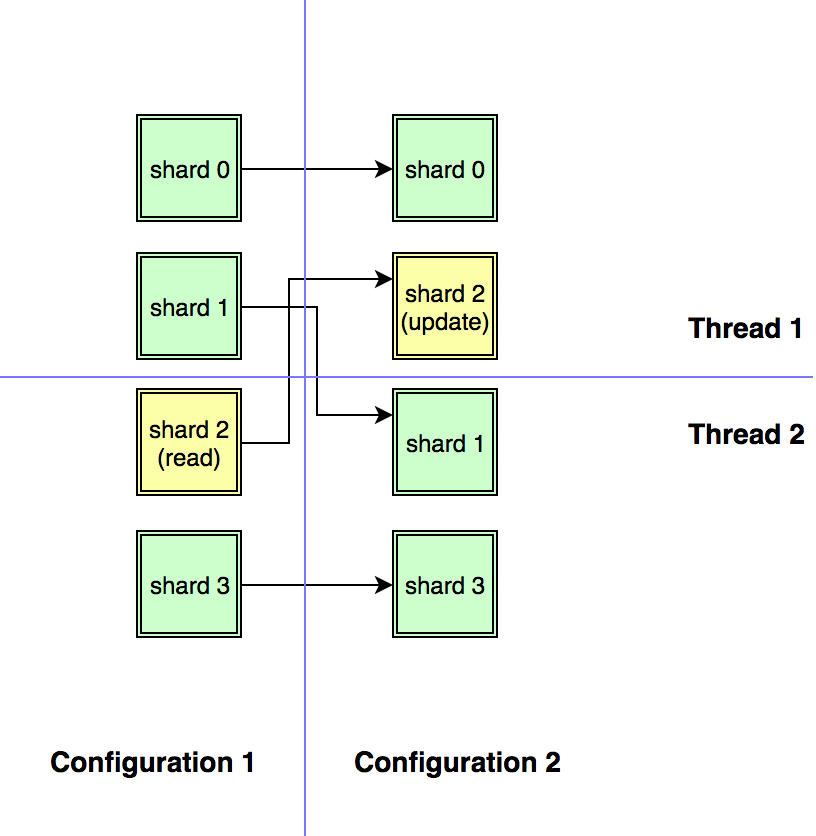
\includegraphics[width=0.5 \textwidth]{image6.png}\end{center}

In the picture above we may see two configurations. Old configuration shows that shards 0 and 1 belong to thread 1 and shards 2 and 3 belong to thread 2. Next resharded configuration show that shards 0 and 2 belong to thread 1, shards 1 and 3 belong to thread 2. While thread 2 is still using old configuration 1, thread 1 may have already switched to configuration 2. In this very moment thread 1 may start to write updates to shard 2 data, while thread 2 is still reading shard 2 data, which is a data race.

In order to avoid this, we will use mutexes. Mutexes will be locked and released only during $Reshard$ process, which would take place rarely, that is why we do not need to bother about mutexes being slow. More precisely, each shard would be associated with a single mutex. When switching to new sharding configuration, thread releases all the mutexes associated with shards of old configuration, afterwards acquiring all mutexes associated with shards of new configuration.

In the example above, such improvement would result in the fact that thread 1 cannot switch to the new configuration, because it waits mutex associated with shard 2, which is held by thread 2 processing old configuration. Only after thread 2 stops to work with an old configuration, thread 1 may freely start to work with new one.

Mutexes associated with shards help us to solve data races different threads may create. However, another possible problem arises, which is a deadlock. Fortunately, we do not suffer from this problem. Indeed, the only moment when a thread A waits is a point when it tries to lock mutex associated with some specific shard during configuration changing, that is, some other thread B locked that mutex. If thread B has already switched to new sharding configuration, it cannot lock the same shard as thread A, thus such condition is impossible. If thread B still uses old configuration, it is going to switch to a new one and release its locks, stopping to block thread A. That is, we will never have a case of a deadlock.

After coping with algorithmic problems, let us turn to the implementation issues.

$Sharder<Controller>$ contains the following variables:
\begin{itemize}
	\item $controller$ of type $Controller\&$
	\item $first\_conf$ is a vector of vector of shards
	\item $second\_conf$ is a vector of vector of shards
	\item $can\_be\_updated$ (TLS) boolean variable, which specifies if shard data can be modified by $controller$ object
	\item $is\_first\_local$ (TLS) boolean variable, which indicates which configuration a thread is using: $first\_conf$ or $second\_conf$
	\item $thread\_num$ (TLS), which is a current thread number
	\item $reshard\_waiting\_timer$ (TLS) is a $WaitingTimer$ instance needed to measure when next resharding is required (see \fullref{subsec:low_overhead_waiting_timer})
	\item $threads\_count$, which would be initialized on construction
	\item atomic pair $(is\_first\_main, noupdate\_counter)$. $is\_first\_main$ indicates whether current active configuration is stored in $first\_conf$ or in $second\_conf$, while $noupdate\_counter$ shows how many threads promised not to update shards data.
	\item $threads$ is a vector of threads
	\item $shard\_locks$ is a vector of mutexes
\end{itemize}

Data of $Sharder$ is initialized the following way:
\begin{itemize}
	\item $controller$ is initialized by reference, passed to constructor
	\item $threads\_count$ is initialized as minimum of two values: maximum hardware concurrency and $coltronller.GetMaxThreadCount()$
	\item $(is\_first\_main, noupdate\_counter) = (true, 0)$
	\item $first\_conf$ is initialized by call to $controller.GetInitialSharding(thread\_count)$
	\item $second\_conf$ is initialized by default
	\item $threads$ is initialized as an empty vector
	\item $shard\_locks$ is initialized as a vector of size being equal to shards count
	\item for each $thread\_num$ call $controller.OnSwitch(thread\_num, first\_conf[thread\_num])$
\end{itemize}

$Sharder$ would have the following methods:
\begin{itemize}
	\item $GetConf$ accepts boolean and returns $first\_conf$ if $true$ and $second\_conf$ otherwise
	\item $Reshard$
	\item $NoUpdatePromise$
	\item $GetShards$
	\item $SwitchConfiguration$
	\item $ThreadAction$
	\item $Run$
\end{itemize}

$Reshard$ method has the following algorithm:
\begin{itemize}
	\item if it is called not from main thread, do nothing
	\item read $(is\_first\_main, noupdate\_counter)$ pair
	\item if $noupdate\_counter$ is less than $threads\_count$, do nothing. Otherwise, there is a need for resharding
	\item call $controller.GetResharding(GetConf(is\_first\_main), thread\_count)$ catching exceptions
	\item is no exceptions caught, assign result to $GetConf(!is\_first\_main)$, return doing nothing otherwise
	\item try CAS $(is\_first\_main, noupdate\_counter)$ ($(cur\_first\_main, threads\_count) \rightarrow (!cur\_first\_main, 0)$) and do nothing on CAS failure
	\item call $reshard\_waiting\_timer.Reset()$ on CAS success
\end{itemize}

$NoUpdatePromise$ method
\begin{itemize}
	\item sets $can\_be\_updated$ to $false$.
	\item tries to increment $noupdate\_counter$ using CAS and re-reading pair $(is\_first\_main, noupdate\_counter)$ in the cycle until CAS succeeds or until after some of reads we find that $is\_first\_main$ is not the same as $is\_first\_local$.
\end{itemize}

$GetShards$ would have the following logic:
\begin{itemize}
	\item check if $is\_first\_local$ is the same as $is\_first\_main$. If so, we do not need to switch to a new configuration. Otherwise, we need to call $SwitchConfiguration$ method
	\item return $GetConf(is\_first\_local)[thread\_num]$
\end{itemize}

$SwitchConfiguration$ procedure does the following:
\begin{itemize}
	\item call $reshard\_waiting\_timer.Reset()$
	\item for all shards in $GetConf(is\_first\_local)[thread\_num]$ call $unlock$ for the corresponding mutex from $shard\_locks$ vector
	\item for all shards in $GetConf(is\_first\_main)[thread\_num]$ call $lock$ for the corresponding mutex from $shard\_locks$ vector
	\item update $is\_first\_local = is\_first\_main$
	\item set $can\_be\_updated$ to $true$.
	\item call $controller.OnSwitch(thread\_num, GetConf(ls\_first\_local)[thread\_num])$
\end{itemize}

$ThreadAction$ is a function which would be assigned to threads. It accepts $thread\_num$ and does the following:
\begin{itemize}
	\item set TLS variable $thread\_num$ to the value it accepted from caller
	\item call $exception\_top\_keeper.SetPath(...thread\_num...)$ passing some filename, which contains $thread\_num$ (for details refer \fullref{subsec:exception_top_proto_storage_interface})
	\item start an infinite cycle
	\item call $exception\_top\_keeper.WithCatchingException$ passing it lambda function with the forthcoming logic:
	\item call $GetShards$ and store value to $shards$ variable
	\item call $controller.PreProcess(thread\_num, can\_be\_updated)$
	\item for each shard in $shards$ call $controller.ProcessShard(can\_be\_updated, shard\_num)$
	\item if $reshard\_waiting\_timer.CheckTime()$ returns $true$, time for resharding has come. We have to call $NoUpdatePromise$ and $Reshard$.
\end{itemize}

Since $ThreadAction$ calls only functions $SetPath$ and $WithCatchingException$, which do not throw, it also does not throw.

Finally, $Run$ method does the following:
\begin{itemize}
	\item initializes $threads$ vector with $thread\_count - 1$ threads associated with $ThreadAction$
	\item calls $ThreadAction$ in main thread also.
\end{itemize}

Let us also outline the algorithmic and exception requirements to $controller$.

First of all, the algorithmic requirements:
\begin{itemize}
	\item $ProcessShard(can\_be\_updated, shard\_num)$ should manipulate with external not-thread-safe data only if a data is uniquely specified by $shard\_num$ and there is no intersection between different $shard\_num$'s data. Function cannot update such data in case if $can\_be\_updated$ is $false$.
	\item $PreProcess$ cannot manipulate with external not-thread-safe data at all, because it is not protected with mutexes.
	\item $GetResharding$ can safely read all data associated with shards, which was updated during $ProcessShard$ calls. It is also safe to assume, that no other thread calls $OnSwitch$ until $GetResharding$ finishes. That is because before $GetResharding$ call all threads promised not to update current shards info, which means that they are already using current shard configuration and not going to switch until CAS, which goes after $GetResharding$.
	\item while implementing $OnSwitch(thread\_num, new\_shards)$ it is safe to assume, that each shard of $new\_shards$ is not processed by any thread until $OnSwitch$ completion. That is because before calling $OnSwitch$, we locked the shards in the current thread, but have not started to process them yet. It is also safe to assume, that main thread is not processing function $GetResharding$ until $OnSwitch$ completion, for the reason that otherwise $OnSwitch$ is processed at the same time as $GetResharding$ is processing, which is impossible as it has been stated above.
\end{itemize}

The exception requirements:
\begin{itemize}
	\item $ProcessShard$ may throw, should provide at least basic exception safety
	\item $PreProcess$ may throw, should provide at least basic exception safety
	\item $OnSwitch$ should not throw
	\item $GetInitialSharding$ may throw, should provide basic exception safety (however, any reasonable implementation would not throw anyway)
	\item $GetResharding$ may throw, should provide at least basic exception safety
	\item $GetMaxThreadCount$ may throw, should provide at least basic exception safety
\end{itemize}

\subsection{Dynamically-sharded message passing pool}

In the section \fullref{subsec:shadow_page_thread_wise_sharder} we have discussed how to shard a job. However, what remained uncovered is how to separate some job into shards and how to do resharding process. In case of a uniform job, for example, calling function $Func$ for each element of some vector, the question of how to shard a job is rather simple. When a job is complicated, it can usually be represented as several distinct logic blocks, some of which use results of some other logical blocks and together they form a full algorithm. That is called a ``message passing''. We would have several distinct message processors, which can accept messages, process them, and send messages to another message processors.

In message passing, a shard would be associated with a message processor. All message processors can be called in different threads if we use thread-safe queue for communication between message processor (sending message processor may be processed in one thread, while receiving message processor may be processed in another thread, which is why we have to use thread-safe queue).

Let us use a queue from the section \fullref{subsec:dealloc_lock_free_queue}.

For thread-safe processing of sharding mechanism, let us use \fullref{subsec:shadow_page_thread_wise_sharder}. It requires shards being associated with integer numbers, which is why we would need some technical coding pattern to map message processor class names into integer numbers. The full idea of how to cope with it is described in \fullref{subsec:specifications_cascade_merging} and \fullref{subsec:reverse_template_instantiation} and a detailed implementation is discussed in \fullref{subsec:message_passing_tree}.

Here we will assume we already know how to map message processor to its integer index and vise versa.

What remains is to define $Controller$ class, which is required in order to use \fullref{subsec:shadow_page_thread_wise_sharder}. Let this class be called $MessagePassingController$.

It would store the following information:
\begin{itemize}
	\item $message\_passing\_tree$ is an instance of $MessagePassingTree$ class designed in the section \fullref{subsec:message_passing_tree}. $MessagePassingTree$ helps to match message passing queues and message processors with their indices.
	\item $message\_wait\_cvs$ is a vector of condition variables. $message\_wait\_cvs$ contains condition variables by a thread number. These condition variables would help to know when message passing queues are not empty. This vector is initialized in the constructor and never changes.
	\item $message\_send\_cvs$ is a vector of pointers on same condition variables, indexed by outgoing message passing queues. It would help to notify condition variables on sending messages. The vector has to be rebuilt on each resharding.
	\item $are\_queues\_empty$ (TLS) boolean variable which specifies whether incoming message queues have been empty on previous step
	\item static constant $wait\_for\_messages\_time$ which specifies how much time a thread waits for message passing queues not to be empty in case all queues was empty at the previous step
	\item vector $message\_processor\_timers$ of $StartFinishTimer$ instances for each message processor
	\item vector $edge\_timers$ of $StartFinishTimer$ instances for each queue.
\end{itemize}

Now let us turn to the implementation of $Controller$ required functions.

$GetMaxThreadCount$ does the following:
\begin{itemize}
	\item returns total number of message processors, which we can get using\\
		$message\_passing\_tree.GetMessageProcessorsCount()$
\end{itemize}

$PreProcess(thread\_num, can\_be\_updated)$ does the following:
\begin{itemize}
	\item if $are\_queues\_empty$ is true, waits for $wait\_for\_messages\_time$,\\
		interrupting on $message\_wait\_cvs[thread\_num]$ condition variable notification. We will use dumb lock instead of mutex while waiting for condition variable as far as there would be nothing terrible if we miss a wake, because we wait for it a very limited amount of time. Condition variable is needed here merely to interrupt waiting earlier if possible.
	\item sets $are\_queues\_empty$ to $true$
\end{itemize}

$ProcessShard(can\_be\_updated, shard\_num)$ does the following:
\nopagebreak
\begin{itemize}
	\item if $can\_be\_updated$ is $true$, calls $message\_processor\_timers[shard\_num].Start()$
	\item using $message\_passing\_tree$ calls $Ping$ method for message processors with index $shard\_num$
	\item if $can\_be\_updated$ is $true$, calls $message\_processor\_timers[shard\_num].Finish()$
	\item gets all incoming queues indices using \\
		$message\_passing\_tree.GetIncomingEdges(shard\_num)$
	\item if $can\_be\_updated$ is $true$ for each index $queue\_index$ calls \\
		$edge\_timers[queue\_index].Start()$
	\item calls $message\_passing\_tree.GetEdgeProxy(queue\_index).NotifyAboutMessage()$
	\item if $can\_be\_updated$ is $true$ calls $edge\_timers[queue\_index].Finish()$
	\item if any message passing queue was not empty, sets $are\_queues\_empty$ to $false$
\end{itemize}

Additional helper function $SetSenderCVs$ would accept vector of vector of shards and do the following:
\begin{itemize}
	\item calculate max queue index by $message\_passing\_tree.GetEdgesCount()$
	\item for all indices $cur\_queue\_index$ get receiver index by calling\\
		$message\_passing\_tree.GetEdgeProxy(cur\_queue\_index).GetToIndex()$
	\item find out a number of thread $thread\_num$, which is going to process this receiver
	\item save pointer to condition variable $message\_wait\_cvs[thread\_num]$ \\ to the location $message\_send\_cvs[cur\_queue\_index]$
\end{itemize}

$GetInitialSharding(thread\_count)$ does the following:
\begin{itemize}
	\item gets a total number of message processors from \\
		$message\_passing\_tree.GetMessageProcessorsCount()$ and distributes them among threads by modulo, returning required vector of vectors
	\item calls $SetSenderCVs$ passing vector of vector of shards
\end{itemize}

$OnSwitch(thread\_num, new\_shards)$ does the following:
\begin{itemize}
	\item for each $new\_shard$ in $new\_shards$ calls \\
		$message\_passing\_tree.GetOutgoingEdges(new\_shard)$ to get outgoing queues indices
	\item for all outgoing queues sets condition variable of queue (by calling $SetConditionVariable$ method) to $message\_send\_cvs[outgoing\_queue\_index]$. As far as no $ProcessShard$ on any current message processor is processing, we may safely update condition variables of outgoing queues facing no data races.
	\item calls $message\_processor\_timers[new\_shard].Reset()$
	\item gets all incoming edges indices by call to \\
		$message\_passing\_tree.GetIncomingEdges(new\_shard)$
	\item calls  $edge\_timers[incoming\_edge\_index].Reset()$
\end{itemize}

In order to define $GetResharding$ procedure, let us introduce several local variables it is going to use:
\begin{itemize}
	\item $chosen\_processors$ is a vector of message processor indices chosen to be processed by current thread we consider
	\item $chosen\_duration$ is a sum of durations of $Ping$ and $Receive$ calls of chosen message processors
	\item $durations$ is a set of pairs $(duration, message\_processor\_index)$ where $duration$ is a sum of durations of $Ping$ and $Receive$ calls of a corresponding message processor with index $message\_processor\_index$
	\item $passing\_durations$ is a hashmap, which by $message\_processor\_index$ stores sum of durations of $Receive$ methods, associated with edges connecting message processor with index $message\_processor\_index$ with message processors from $chosen\_processors$
\end{itemize}

Let us introduce helping procedure $ChoozeProcessor$ which accepts all variables defined above ass well as a pair $(duration, message\_processor\_index)$ and is going to add a \\
$message\_processor\_index$ to $chosen\_processors$ and update all the variables listed the following way:
\begin{itemize}
	\item increment $chosen\_duration$ by $duration$
	\item delete pair $(duration, message\_processor\_index)$ from $durations$
	\item for each $other\_message\_processor\_index$ remained in $durations$ pairs find index of edges between message processor with index $message\_processor\_index$ and message processor with index $other\_message\_processor\_index$ by the call to \\
		$message\_passing\_tree.GetConnectingEdges$
	\item for each found $edge\_index$ increment \\
		$passing\_durations[other\_message\_processor\_index]$ by the result of \\
		$edge\_timers[edge\_index].GetDurationSum()$ call
\end{itemize}

$GetResharding(shard\_configuration, thread\_count)$ does the following:
\begin{itemize}
	\item calculates sum of all $GetDurationSum$ values from times in $message\_processor\_timers$ and in $edge\_timers$ as well
	\item divides sum by $thread\_count$ and saves result to local variable $avg\_duration$
	\item initializes $durations$ as set of pairs $(duration, message\_processor\_index)$,\\
		where $duration$ is sum of the result of \\
		$message\_processor\_timers[message\_processor\_index].GetDurationSum()$ call
		and the result of \\
		$edge\_timers[edge\_index].GetDurationSum()$ call for each $edge\_index$ of incoming edge
	\item starts a cycle A for each $thread\_num$ from 0 to $thread\_count - 1$
	\item initializes $chosen\_duration = 0$
	\item initializes $chosen\_processors$ as an empty vector
	\item initializes $passing\_durations$ is an empty hashmap
	\item if maximum duration in $durations$ is more than $avg\_duration$, calls $ChoozeProcessor$ for corresponding pair in $durations$ set.
	\item starts a while cycle B until $durations$ is not empty
	\item by means of binary search finds in the set $durations$ an upper bound of durations, which can be added to $chosen\_duration$ so that sum is not more than $avg\_duration$. That is, we want to add message processors until sum of their execution durations does not exceed average wanted time.
	\item if there are no such durations in $durations$ set, there is no message processor we can add to the current thread without exceeding average execution time. In this case, algorithm breaks cycle B.
	\item In the other case, among all suitable message processors with duration less than found upper bound, chooses a $message\_processor$, which has the largest passing duration, which is detected by $passing\_durations$ hash map (absence of key in $passing\_durations$ map implies zero value here)
	\item calls $ChoozeProcessor$
	\item goes to the start of B cycle
	\item if got here, algorithm has nothing more to add to the current thread
	\item adds $chosen\_processors$ to vector of vector of shards we are going to return from this function
	\item goes to the start of A cycle
	\item calls $SetSenderCVs$ for just built vector of vector of shards
	\item returns vector of vector of shards
\end{itemize}

Such algorithm helps to distribute computations evenly and also tries to combine message processors with high communication rate together, which helps to reduce cache ping-pong while two message processors are accessing the same message passing queue.

Let us check that we work with data correctly, without any races. In order to do that, we have to consider every variable we store:
\begin{itemize}
	\item $message\_passing\_tree$ is a proxy object made to access queues and message processors, it is not modified itself
	\item $message\_wait\_cvs$ is not modified after initialization
	\item $message\_send\_cvs$ is accessed in several functions: $SetSenderCVs$ which is called inside resharding, also it is accessed in $OnSwitch$. Sharder guarantees $OnSwitch$ never intersects with resharding in execution timeline.
	\item $are\_queues\_empty$ is in TLS, thus no races are possible
	\item $wait\_for\_messages\_time$ is constant
	\item $message\_processor\_timers$ is accessed in several functions: $ProcessShard$ updates $shard\_num$ index, $OnSwitch$ updates indices of switching shards, $GetResharding$ reads the whole vector. In order to sort it out, let us consider all pairs of functions. First of all, sharder guarantees that shards passed to $OnSwitch$ are not processed by $ProcessShard$ at the moment of $OnSwitch$ execution, which implies, that there is no race between $OnSwitch$ and $ProcessShard$. Secondly, $ProcessShard$ does not update information read by $GetResharding$ because of $NoUpdatePromise$ requirement. Finally, $OnSwitch$ and $GetResharding$ have not intersecting execution timelines, that is why they do not conflict either.
	\item $edge\_timers$ is accessed in several functions: $ProcessShard$ updates indices, which are incoming queue indices for message processor $shard\_num$, $OnSwitch$ also accesses only indices of incoming queues of its shards, $GetResharding$ accesses the whole vector. The same discourse as above would show that there are no data races.
\end{itemize}

As it can easily be concluded, we do not have data races in $MessagePassingController$.

\begin{samepage}
	The only question remained is whether in satisfies $Sharder$ requirements on $Controller$ class:
	\begin{itemize}
		\item $ProcessShard$ manipulates with message processor indexed by $shard\_num$ and its incoming queues. It is obvious that these objects sets do not intersect for different shard numbers.
		\item $PreProcess$ manipulates with thread-safe condition variable and TLS variable\\
			$are\_queues\_empty$, which is ok
		\item $OnSwitch$ does not throw, it calls only noexcept functions
		\item the rest functions have basic exception safety
	\end{itemize}
\end{samepage}
All the requirements of sharder are satisfied.

\subsection{Increasing hex identifier}
\label{subsec:increasing_hex_identifier}

This is simply an algorithm for generating string identifiers of the form f12f-abc3-12a4. We want our $HexIdGenerator$ to have increment method, which increments the identifier, and $GetHex$ method, which returns generated string. Strings should increase lexicographically on each increment.

In order to do that let us introduce $HexToken$ class, which contains the following fields:
\begin{itemize}
	\item $index$ is a 16-byte integer number
	\item $hex\_repr$ is a hex representation string
\end{itemize}

$HexToken$ would have the following methods:
\begin{itemize}
	\item $IsOver$ indicates whether $index$ reached its maximum, which is 65535.
	\item $UpdateHexRepr$, which updates the representation of $index$ in hex string format and stores the result to $hex\_repr$ variable
	\item $GetHex$, which returns reference to string $hex\_repr$
	\item $operator\mbox{++}$, which increments the $index$ and calls $UpdateHexRepr$ to update hex representation
\end{itemize}

Methods $IsOver$ and $GetHex$ would be exception-free. As for the rest, if $UpdateHexRepr$ fails inside $operator\mbox{++}$, $operator\mbox{++}$ would still be retryable, it would increment $index$ again and call $UpdateHexRepr$ on next retrying call. That is, in case of failure we may increment $index$ by 2, missing $index + 1$ representation construction, but this does not break the invariant of increment operation to produce lexicographically larger strings. That is, function provides basic exception safety guarantee.

Now let us consider $HexIdGenerator$, which stores the following information:
\begin{itemize}
	\item $hex\_tokens$ vector of $HexToken$ objects
	\item $hex\_repr$, which stores full hex representation of the identifier
\end{itemize}

$HexIdGenerator$ would have the following functions:
\begin{itemize}
	\item $operator\mbox{++}$, which iterates the identifier
	\item $GetHex$, which returns reference of string $hex\_repr$
\end{itemize}

$operator\mbox{++}$ would have the following algorithm:
\begin{itemize}
	\item iterate through all $hex\_token$ from vector $hex\_tokens$
	\item if $hex\_token.IsOver()$ returns $false$, call $\mbox{++}hex\_token$, fix $hex\_repr$ by calling \\
		$hex\_token.GetHex()$ and placing new hex string to the place in whole $hex\_repr$ where it belongs. Afterwards, return from function
	\item if we reached to the end of the iteration through all $hex\_tokens$, then we have an identifier of the form ffff-ffff-ffff...
	\item append 0000 to $hex\_repr$ if its length is not more, than $5 * hex\_tokes.size() - 1$
	\item add new element to $hex\_tokens$ vector
\end{itemize}

$GetHex$ method of $HexIdGenerator$ would return reference to $hex\_repr$ and do nothing else. This method does not throw.

As for $operator\mbox{++}$, it may throw. There are several cases:
\begin{itemize}
	\item $\mbox{++}hex\_token$ failed. In this case, the length of $hex\_repr$ remained unchanged. While it is unchanged, it consists of fixed amount of strings from $HexToken$, which are guaranteed to increase even in case of failures. That is, $hex\_repr$ also will be guaranteed to increase in this specific case
	\item appending  0000 to $hex\_repr$ failed. In this case, function has no effect
	\item adding new element to $hex\_tokens$ vector failed. In such a case, we would have a string of the form ffff-ffff-ffff-0000 and not updated vector of $hex\_tokens$. On the next retry of $operator\mbox{++}$, it will again find, that all $hex\_tokens$ are over, but this time we will not append 0000 to the $hex\_repr$, because of length check. Afterwards, function would finish appending element of $hex\_tokens$ and the structure would become consistent again.
\end{itemize}

That is, $operator\mbox{++}$ provides basic exception safety.

\newpage
\section{Detailed Code Architecture (classes and methods)}

\subsection{TLS free-list multi-level allocator}

The class implements the allocation logic described in the section \fullref{free_list_algo}.

\begin{lstlisting}
class FreeListMultiLevelAllocator {
	FreeListMultiLevelAllocator()
	// Exceptions:
	// 	may throw, strong exception safety

	FreeListMultiLevelAllocator(
		const FreeListMultiLevelAllocator&) = delete;

	FreeListMultiLevelAllocator(
		FreeListMultiLevelAllocator&&) = delete;

	FreeListMultiLevelAllocator& operator=(
		const FreeListMultiLevelAllocator&) = delete;
	// We will use object as s singleton, no copying and assigning

	template <typename T>
	T* Allocate(const size_t size);
	// Return value:
	// 	a pointer to allocated block
	// Exceptions:
	// 	may throw std::bad_alloc
	// 	strong exception safety: no side effects in exception case

	template <typename T>
	void Deallocate(T* pointer, const size_t size) noexcept;
};

thread_local FreeListMultiLevelAllocator global_allocator;
// Memory allocations would be controlled by this TLS singleton

template <typename T>
class FixedFreeListMultiLevelAllocator<T> {
	FixedFreeListMultiLevelAllocator() noexcept;

	FixedFreeListMultiLevelAllocator(
		const FixedFreeListMultiLevelAllocator&) noexcept;

	template <class U>
	FixedFreeListMultiLevelAllocator(
		const FixedFreeListMultiLevelAllocator<U>&) noexcept;
	// These three methods are empty,
	// 	they are needed for compatibility with std::allocator

	T* allocate(const size_t n);
	// Calls global_allocator.Allocate<T>(n)
	// Return value:
	// 	a pointer to allocated block
	// Exceptions:
	// 	may throw std::bad_alloc
	// 	strong exception safety: no side effects in exception case

	void deallocate(T* p, const size_t n) noexcept;
	// Calls global_allocator.Deallocate<T>(p, n)
};
\end{lstlisting}

\subsection{Lock-free queue}

$LockFreeQueue<TElement>$ is an implementation of lock-free queue described in the section \fullref{subsec:dealloc_lock_free_queue}. It contains the following functions:

\begin{lstlisting}
class LockFreeQueue<TElement> {
	void Push(TElement new_element);
	// Exceptions:
	// 	Strong exception safety: in case of failure
	// 	the element is not pushed to the queue,
	// 	there are no visible side effects

	std::unqiue_ptr<TElement> Pop() noexcept;
	// Return value:
	// 	nullptr unique_ptr if the queue was empty,
	// 	unique_ptr pointing on TElement in case of successful pop
};
\end{lstlisting}

\subsection{Message processor}
\label{subsec:message_processor}
Message processor is a class with $Ping$ method, which is called periodically, and $Receive$ method, which is called on receiving a message from another message processor. Both methods accept object $sender$ of unspecified type and may use it in order to send messages to another message processors.

All message processors have base class $MessageProcessorBase$:

\begin{lstlisting}
class MessageProcessorBase {
public:
	template <typename Sender>
	void Ping(const Sender&) {}
	// Empty method, needed if we do not want to define corresponding Ping method in child class

	virtual ~MessageProcessorBase() noexcept {}
};
\end{lstlisting}

All message processors look like this:
\begin{lstlisting}
class MessageProcessor : public MessageProcessorBase {
public:
	using MessageProcessorBase::MessageProcessorBase;

	template <typename Sender>
	void Ping(const Sender& sender) {
		// here a call to sender.template Send<YetAnotherMessageProcessor>(new AnotherMessageType())
		// may be or may not be present
	}
	// Ping method may be absent here
	// Exceptions: basic exception safety

	template <typename Sender>
	void Receive(const ReceivingFrom<AnotherMessageProcessor>&, const MessageType& message, const Sender& sender) {
		// here a call to sender.template Send<YetAnotherMessageProcessor>(new AnotherMessageType())
		// may be or may not be present
	}
	// Exceptions: basic exception safety
};
\end{lstlisting}
%TODO check exception safety afterwards
In here $ReceivingFrom$ is a specification helper dumb class:
\begin{lstlisting}
template <typename T>
class ReceivingFrom {};
\end{lstlisting}
This class is needed to specify several Receive methods in the $MessageProcessor$ in order to specialize, from which $AnotherMessageProcessor$ are we receiving a message.

$MessageType$ is an arbitrary class, which stores the message itself.

$Sender$ is a template parameter, which is needed for the reason that sender object is of an unspecified type.

\subsection{Message passing tree}
\label{subsec:message_passing_tree}

$MessagePassingTree<Edge<MessageProcessor1, MessageProcessor2, MessageType1>, Edge<MessageProcessor3, MessageProcessor4, MessageType2>, ...>$ is a message-processor controller. It helps to register message passing communication edges and check are there unregistered send operations inside \hyperref[subsec:message_processor]{message processors} at a compile time. Additionally, it stores message passing queues, which help to send messages from one message processor to another.

Moreover, this class provides an opportunity to access distinct message processors by index as well as access message queues by their indices. Furthermore, it can tell which indices of message queues are connected with which message processor indices.

Hence, this is  a generic structure which controls message passing process and provides access by indices, which simplifies further programming.

The structure here is rather complicated and based on the \fullref{subsec:specifications_cascade_merging} and \fullref{subsec:reverse_template_instantiation} patterns.

First of all, there is a zero-template very-base class $Piper<>$ definition:
\begin{lstlisting}
template <typename ... Args>
class Piper {
protected:
	template <typename GlobalPiper>
	class EdgeProxy {
	public:
		EdgeProxy(GlobalPiper& piper) noexcept;
		// Remembers piper reference

		virtual bool NotifyAboutMessage() const = 0;
		virtual void SetConditionVariable(std::condition_variable_any *) const noexcept = 0;
		virtual const int GetFromIndex() const noexcept = 0;
		virtual const int GetToIndex() const noexcept = 0;

		virtual ~EdgeProxy() noexcept {}
	protected:
		GlobalPiper& piper;
	};

	template <typename GlobalPiper>
	class MessageProcessorProxy {
	public:
		MessageProcessorProxy(GlobalPiper& piper, const int message_processor_index) noexcept;
		// init piper and message_processor_index

		template <typename MP>
		MP& GetMessageProcessor() const noexcept;
		// Returns MessageProcessor instance
	protected:
		GlobalPiper& piper;
		int message_processor_index;
	}
public:
	Piper() noexcept;
	// initializes max_message_processor_index and max_edge_index as zero

	template <typename MP>
	int GetMessageProcessorIndexImpl(const TypeSpecifier<MP>&) noexcept;
	// returns -1

	template <typename GlobalPiper>
	void FillEdgeProxysImpl(GlobalPiper&, std::vector<std::unique_ptr<Piper::EdgeProxy<GlobalPiper>>>&);
	// Empty function
	// May throw, basic exception safety

	void GetEdgeIndexImpl() noexcept;
	// Empty function

	template <typename GlobalPiper>
	void AddMessageProcessorsImpl(GlobalPiper&,
		std::vector<std::unique_ptr<Piper::MessageProcessorProxy<GlobalPiper>>>&);
	// Empty function
	// May throw, basic exception safety

	virtual ~Piper();
protected:
	int max_message_processor_index;
	int max_edge_index;
	std::vector<std::vector<int>> dest_pipes;
	std::vector<LockFreeQueue<std::unique_ptr<MessageBase>>> queues;
	std::vector<std::unique_ptr<MessageProcessorBase>> message_processors;
};
\end{lstlisting}

Now the definition of a complete inherited class
\begin{lstlisting}
template <typename From, typename To, typename Message, typename ... Args>
class Piper<Edge<From, To, Message>, Args...> : public Piper<Args...> {
protected:
	template <typename GlobalPiper, typename From2>
	class SenderProxy {
	// Sender class for MessageProcessors.
	// GlobalPiper is a last Piper<...> child class in the inheritance chain
	public:
		SenderProxy(GlobalPiper& piper) noexcept;
		// Initialize piper reference

		template <typename To2, typename Message2>
		void Send(std::unique_ptr<Message2> message);
		// notifies condition variable from notify_condition_variables vector
		// May throw, strong exception safety
	private:
		GlobalPiper& piper;
	};

	template <typename GlobalPiper, typename MP>
	class MessageProcessorProxy : public Piper<>::MessageProcessorProxy<GlobalPiper> {
	public:
		using Piper<>::MessageProcessorProxy<GlobalPiper>::MessageProcessorProxy;
		using Piper<>::MessageProcessorProxy<GlobalPiper>::piper;

		virtual void Ping() const;
		// Calls MessageProcessor Ping method, passing a SenderProxy object
		// May throw, basic exception safety

	};

	template <typename GlobalPiper>
	class EdgeProxy : public Piper<>::EdgeProxy<GlobalPiper> {
	public:
		using Piper<>::EdgeProxy<GlobalPiper>::EdgeProxy;
		using Piper<>::EdgeProxy<GlobalPiper>::piper;

		virtual bool NotifyAboutMessage() const;
		// if queue is not empty, calls Receive method of MessageProcessor, passing as SenderProxy object
		//	and returns true, returns false otherwise
		// May throw, basic exception safety

		virtual void SetConditionVariable(std::condition_variable_any*) const noexcept;
		// sets corresponding condition variable in vector notify_condition_variables

		virtual const int GetFromIndex() const noexcept;
		// returns cur_to_index of current Piper layer

		virtual const int GetToIndex() const noexcept;
		// returns cur_from_index of current Piper layer

	};
public:
	using Piper<Args...>::max_message_processor_index;
	using Piper<Args...>::GetMessageProcessorIndexImpl;
	using Piper<Args...>::max_edge_index;
	using Piper<Args...>::dest_pipes;
	using Piper<Args...>::queues;
	using Piper<Args...>::message_processors;
	using Piper<Args...>::GetEdgeIndexImpl;

	Piper() noexcept;
	// Does nothing

	template <typename GlobalPiper, typename MP>
	void AddMessageProcessorIfNotExists(int& target_index,
		GlobalPiper& piper,
		std::vector<std::unique_ptr<Piper<>::MessageProcessorProxy<GlobalPiper>>>& message_processor_handlers
		const bool is_to);
	// Calls GetMessageProcessorIndexImpl to find MP's message processor index. If returns -1
	// 	(from a base Piper class implementation), nothing found. In this case function generates new
	//	message processor index (target_index = max_message_processor_index++) and pushes a new instance
	//	of MessageProcessor to message_processors and
	//	a new instance of MessageProcessorProxy<GlobalPiper, MP> to message_processor_handlers,
	//	passing current new generated index of message processor to constructor of MessageProcessorProxy.
	//	Also it pushes new empty vector to dest_pipes.
	//	In any case it saves old or new generated message processor index to target_index.
	// May throw, basic exception safety

	template <typename GlobalPiper>
	void AddMessageProcessorsImpl(GlobalPiper& piper,
		std::vector<std::unique_ptr<Piper<>::MessageProcessorProxy<GlobalPiper>>>& message_processor_handlers);
	// Calls itself for parent class,
	//	then calls AddMessageProcessorIfNotExists for 'From' and for 'To' Message Processor.
	//	Generates cur_edge_index (cur_edge_index = max_edge_index++)
	//	Appends to dest_pipes and queues
	// May throw, basic exception safety

	template <typename GlobalPiper>
	void FillEdgeProxysImpl(GlobalPiper& piper, std::vector<std::unique_ptr<Piper<>::EdgeProxy<GlobalPiper>>>& edge_handlers);
	// Calls itself for parent class
	//	Fills edge_handlers with EdgeProxy<GlobalPiper> instance
	// May throw, basic exception safety

	void InitializeNotifyConditionVariables();
	// Initializes notify_condition_variables with nullptrs
	// May throw, basic exception safety


	int GetMessageProciessorIndexImpl(const TypeSpecifier<From>&) noexcept;
	// Specification which returns index of message processor 'From'

	int GetMessageProcessorIndexImpl(const TypeSpecifier<To>&) noexcept;
	// Specification which returns index of message processor 'To'

	int GetEdgeIndexImpl(const TypeSpecifier<Edge<From, To, Message>>&) noexcept;
	// Specification which returns index of edge
private:
	int cur_to_index;
	int cur_from_index;
	int cur_edge_index;
	std::vector<std::condition_variable_any *> notify_condition_variables;
};
\end{lstlisting}

And finally, an enclosing class $MessagePassingTree$, which does all the lazy initialization and provides access to proxy objects:
\begin{lstlisting}
template <typename ... Args>
class MessagePassingTree : public Piper<Args...> {
private:
	using GlobalPiper = Piper<Args...>;
public:
	using GlobalPiper::dest_pipes;

	MessagePassingTree();
	// Calls AddMessageProcessorsImpl<GlobalPiper> to fill message_processor_handlers
	//	calls FillEdgeProxysImpl<GlobalPiper> to fill edge_handlers
	//	calls InitializeNotifyConditionVariables to fill condition variables
	//
	// May throw, basic exception safety

	const Piper<>::EdgeProxy<GlobalPiper>* GetEdgeProxy(const int index) noexcept;
	// returns edge handler from edge_handlers vector

	const Piper<>::MessageProcessorProxy<GlobalPiper>* GetMessageProcessorProxy(const int index) noexcept;
	// returns message processor handler from message_processor_handlers vector;

	const size_t GetMessageProcessorsCount() noexcept;
	// returns message_processor_handlers size

	const size_t GetEdgesCount() noexcept;
	// returns edge_handlers size

	std::vector<int>& GetIncomingEdges(const int message_processor_index) noexcept;
	// Gets all incoming edges

	std::vector<int>& GetOutgoingEdges(const int message_processor_index) noexcept;
	// Gets all outgoing edges

	std::vector<int>& GetConnectingEdges(const int first_mp_index, const int second_mp_index) noexcept;
private:
	std::vector<std::unique_ptr<Piper<>::EdgeProxy<GlobalPiper>>> edge_handers;
	std::vector<std::unique_ptr<Piper<>::MessageProcessorProxy<GlobalPiper>>> message_processor_handlers;
};
\end{lstlisting}

\subsection{Low-overhead timers}

Let us outline classes and methods for several algorithms described above:
\begin{itemize}
	\item \fullref{subsec:low_overhead_periodic_timer}
	\item \fullref{subsec:low_overhead_start_finish_timer}
	\item \fullref{subsec:low_overhead_waiting_timer}
	\item \fullref{subsec:low_overhead_periodic_clock}
\end{itemize}

\begin{lstlisting}
class PeriodicTimer {
private:
	void WindUp() noexcept;
public:
	int64_t GetPassedTime() noexcept;
	void Reset() noexcept;
private:
	static const int64_t min_system_click_call_period;
	static const int64_t max_wind_up_steps;
	static const int64_t min_measured_time;
	int64_t wind_up_counter;
	int64_t wind_up_balance;
	int64_t last_wind_up_counter;
	int64_t last_system_time;
	int64_t approx_time_step;
};
class StartFinishTimer {
public:
	void Start() noexcept;
	void Finish() noexcept;
	uint64_t GetCount() noexcept;
	int64_t GetDurationSum() noexcept;
	void Reset() noexcept;
private:
	PeriodicTimer start_timer;
	PeriodicTimer finish_timer;
	uint64_t measurements_counter;
	int64_t duration_sum;
};
class WaitingTimer {
public:
	WaitingTimer(const uint64_t time_period) noexcept;
	bool CheckTime() noexcept;
	void Reset() noexcept;
private:
	uint64_t time_period;
	int64_t time_elapsed;
	PeriodicTimer periodic_timer;
};
class PeriodicClock {
public:
	int64_t GetTime() const noexcept;
private:
	PeriodicTimer periodic_timer;
	int64_t current_time;
};
\end{lstlisting}

\subsection{Exception with backtrace}
\label{subsec:exception_with_backtrace}

For various reasons, while handling exception, one may want to get access to stacktrace. For instance, having stacktrace makes it possible to pass it to the user, without aborting the program.

Let us introduce a class $ExceptionWithBacktrace$ which on construction will accept exception reason as string and will remember current stacktrace from place in the code it was constructed. Moreover, it would register itself in global $exception\_top\_keeper$ instance.

Let the $ExceptionWithBacktrace$ class be the following:
\begin{lstlisting}
class ExceptionWithBacktrace : public std::exception {
public:
	ExceptionWithBacktrace(const std::string& reason) noexcept
	// stores reason and current backtrace, and their
	//	human-readable concatenation in reason_with_backtrace,
	//	catches inner exceptions and if caught, may leave
	//	some of inner string fields empty

	const std::string& GetStackStrace() const noexcept;
	// returns backtrace;

	const char* what() const noexcept;
	// return reason_with_backtrace.c_str()

	const std::string& GetReasonWithBacktrace() const noexcept;
	// returns reason_with_backtrace
private:
	std::string reason;
	std::string backtrace;
	std::string reason_with_backtrace;
};
\end{lstlisting}

\subsection{Exception top proto storage interface}
\label{subsec:exception_top_proto_storage_interface}
Here we are to outline classes and methods of $ExceptionTopKeeper$, which is defined in the section \fullref{subsec:exception_top_proto_storage}.

\begin{lstlisting}
class ExceptionTopKeeper {
public:
	void Dump() const noexcept;

	void Restore();

	void Trim() noexcept;

	void RemoveOld(const int64_t current_time) noexcept;

	void SetPath(const std::string& new_path) noexcept;

	template <typename Function>
	void WithCatchingException(Function func) noexcept;
private:
	std::string path;
	std::unordered_map<std::string, uint64_t> exception_frequency;
	std::unordered_map<std::string, int64_t> exception_last_time;
	std::set<std::pair<uint64_t, std::string>> frequency_exception;
	std::set<std::pair<int64_t, std::string>> last_time_exception;
	WaitingTimer dump_timer;
	PeriodicClock store_clock;
	static const size_t top_size;
	static const int64_t keep_time;
	static const debug_mode;
}
\end{lstlisting}

Let us also declare a global thread\_local instance of the class above

\begin{lstlisting}
thread_local ExceptionTopKeeper exception_top_keeper;
\end{lstlisting}
\subsection{Shadow-paging thread-wise sharder interface}
Here we are to outline classes and methods required for $Sharder$, which is described in the section \fullref{subsec:shadow_page_thread_wise_sharder}

Here is how helper class looks
\begin{lstlisting}
class Controller {
public:
	void ProcessShard(const bool can_be_updated, const int shard_num);
	// Exceptions: basic safety

	void PreProcess(const int thread_num, const bool can_be_updated);
	// Exceptions: basic safety

	void OnSwitch(const int thread_num, const std::vector<int>& new_shards) noexcept;

	std::vector<std::vector<int>> GetInitialSharding(cont int thread_count);
	// Exceptions: basic safety

	std::vector<std::vector<int>> GetResharding(
		const std::vector<std::vector<int>>& old_shard_configuration,
		const int thread_count);
	// Exceptions: basic safety

	const int GetMaxThreadCount();
	// Exceptions: basic safety
};
\end{lstlisting}

Now let us define $Sharder$ class itself:
\begin{lstlisting}
struct ShadowCounter {
	bool is_first_main;
	unsigned noupdate_counter:7;
};

template <typename Controller>
class Sharder {
public:
	Sharder(Controller& controller);
	// Constructor may throw, basic exception safety

	std::vector<std::vector<int>>& GetConf(bool is_first) noexcept;

	void Reshard() noexcept;

	void NoUpdatePromise() noexcept;

	std::vector<int>& GetShards() noexcept;

	void SwitchConfiguration() noexcept;

	void ThreadAction(const int thread\_num) noexcept;
	// Inside we have to catch exceptions, though

	void Run() noexcept;
	// Thread launching may throw, but if it does, we cannot do anything better than to terminate
	// That is why we mark function as noexcept
private:
	std::vector<std::vector<int>> first_conf;
	std::vector<std::vector<int>> second_conf;
	int threads_count;
	ShadowCounter shadow_counter;
	std::vector<std::thread> threads;
	std::vector<std::mutex> shard_locks;

	static thread_local bool can_be_updated;
	static thread_local bool is_first_local;
	static thread_local int thread_num;
	static thread_local WaitingTimer reshard_waiting_timer;
};
\end{lstlisting}

\subsection{Dynamically-sharded message passing pool interface}
Controller object have the following interface:
\begin{lstlisting}
template <typename ... Args>
class MessagePassingController {
public:
	MessagePassingController();
	// Exceptions: basic safety

	void ProcessShard(const bool can_be_updated, const int shard_num);
	// Exceptions: basic safety

	void PreProcess(const int thread_num, const bool can_be_updated);
	// Exceptions: basic safety

	void OnSwitch(const int thread_num, const std::vector<int>& new_shards) noexcept;

	std::vector<std::vector<int>> GetInitialSharding(cont int thread_count);
	// Exceptions: basic safety

	std::vector<std::vector<int>> GetResharding(
		const std::vector<std::vector<int>>& old_shard_configuration,
		const int thread_count);
	// Exceptions: basic safety

	const int GetMaxThreadCount();
	// Exceptions: basic safety
private:
	MessagePassingTree<Args...> message_passing_tree;
	std::vector<std::condition_variable_any> message_wait_cvs;
	std::vector<std::condition_variable_any *> message_send_cvs;
	static thread_local bool are_queues_empty;
	static const uint64_t wait_for_messages_time;
	std::vector<StartFinishTimer> message_processor_timers;
	std::vector<StartFinishTimer> edge_timers;
};
\end{lstlisting}

Let us also introduce easy-to-use completion wrapper:
\begin{lstlisting}
template <typename ... Args>
class DSMPPool {
public:
	DynamicallyShardedMessagePassing()
	// creates controller by default constructor,
	// 	creates sharder passing controller reference
	// Exceptions: basic safety

	void Run() noexcept;
	// Proxies sharder.Run() call

private:
	MessagePassingController<Args...> controller;
	Sharder<MessagePassingController<Args...>> sharder;
};
\end{lstlisting}
\subsection{Increasing hex identifier interface}

Here we are to outline an interface for \fullref{subsec:increasing_hex_identifier}

\begin{lstlisting}
class HexToken {
private:
	void UpdateHexRepr();
public:
	bool IsOver() const noexcept;

	const std::string& GetHex() const noexcept;

	HexToken& operator++();
	// May throw, basic exception safety is provided
private:
	uint16_t index;
	std::string hex_repr;
};

class HexIdGenerator {
public:
	const std::string& GetHex() const noexcept;

	HexIdGenerator& operator++();
	// May throw, basic exception safety is provided
private:
	std::vector<HexToken> hex_tokens;
	std::string hex_repr;
};
\end{lstlisting}

\end{document}
